%!TEX TS-program = pdflatex
% dissertation.tex -- main dissertation file
%
% Wisconsin dissertation template
% Copyright (c) 2008-2009 William C. Benton.  All rights reserved.
%
% This program can redistributed and/or modified under the terms
% of the LaTeX Project Public License Distributed from CTAN
% archives in directory macros/latex/base/lppl.txt; either
% version 1 of the License, or (at your option) any later version.
%
% This program includes other software that is licensed under the
% terms of the LPPL and the Perl Artistic License; see README for details.
%
% You, the user, still hold the copyright to any document you produce
% with this software (like your dissertation).
%

%%% You'll want ``oneside'' for the deposit version, but probably not for any versions that don't need to meet the UW requirements
\documentclass[12pt,oneside,letterpaper]{memoir}

\usepackage{todonotes}
\usepackage[acronym]{glossaries}

% preamble.tex -- packages to include
%
% Wisconsin dissertation template
% Copyright (c) 2008 William C. Benton.  All rights reserved.
%
% This program can redistributed and/or modified under the terms
% of the LaTeX Project Public License Distributed from CTAN
% archives in directory macros/latex/base/lppl.txt; either
% version 1 of the License, or (at your option) any later version.
%
% This program includes other software that is licensed under the
% terms of the LPPL and the Perl Artistic License; see README for details.
%
% You, the user, still hold the copyright to any document you produce
% with this software (like your dissertation).

%% You should use natbib
\IfFileExists{natbib.sty}{%
\usepackage{natbib}%
}{}

%% You probably need appendix, if you want appendices
\IfFileExists{appendix.sty}{%
\usepackage{appendix}%
}{}

%% the spacing in memoir is weird, you'll need to use this
\DisemulatePackage{setspace}
\usepackage[onehalfspacing]{setspace}

%% List setup; the ``hanglist`` environment will allow you to have
%% nicely-typeset enumerated lists (i.e. with the numbers hanging in
%% the margins).  You need at least version 2.1 of enumitem.sty.  If
%% you don't have enumitem installed at all, hanglist will just be an
%% alias for enumerate.
\IfFileExists{enumitem.sty}{%
\usepackage[loadonly]{enumitem}[2007/06/30]%
\newlist{hanglist}{enumerate}{1}% 
\setlist[hanglist]{label=\arabic*.}%
\setlist[hanglist,1]{leftmargin=0pt}%
}{%
\newenvironment{hanglist}{\begin{enumerate}}{\end{enumerate}}%
}

%% Comment out any of these that you don't want
\usepackage{amssymb}
\usepackage{amsmath}
\usepackage{amsthm}
%\usepackage{theorem}
\usepackage{hyperref}

\IfFileExists{mathpartir.sty}{%
\usepackage{mathpartir}%
}{}

%%%%% LISTINGS package and setup
\IfFileExists{listings.sty}{%
\usepackage{listings}%
}{}



%% Get rid of ugly borders around PDF hyperlinks (e.g. for cross-references, bib entries, or URLs)
\hypersetup{pdfborder = 0 0 0}

%% You want microtype.
\IfFileExists{microtype.sty}{%
\usepackage[protrusion=true,expansion=true]{microtype}%
}{}

%\pagestyle{thesisdraft}

% Surround parts of graphics with box
\usepackage{boxedminipage}

%% booktabs (thx to Nate Rosenblum for bringing this beautiful package
%% to my attention)
\IfFileExists{booktabs.sty}{%
\usepackage{booktabs}%
}{}

% This is now the recommended way for checking for PDFLaTeX:
\usepackage{ifpdf}

%% Avoid ugly "Type 3" fonts
\usepackage{lmodern}
\usepackage[LY1]{fontenc}

%% Substitute your favorite serif and sans fonts here....
\IfFileExists{tgpagella.sty}{%
% TeX Gyre pagella, like Palatino
\usepackage{tgpagella}%
}{}

\usepackage[LY1]{eulervm}

\ifpdf
\usepackage[pdftex]{graphicx}
\else
\usepackage{graphicx}
\fi

\usepackage{makeidx}
\makeindex

{\theoremstyle{plain}
\newtheorem{thm}{Theorem}[chapter]
\newtheorem{cor}[thm]{Corollary}
\newtheorem{define}[thm]{Definition}
\newtheorem{exmpl}[thm]{Example}
}
{\theoremstyle{remark}
\newtheorem{rmk}[thm]{Remark}
}

\newtheoremstyle{customsty1}
{3pt}%
{3pt}%
{}% --- body font
{}% --- indent amount
{\bfseries}% --- Theorem head font
{:}% --- Punctuation after head
{.5em}% --- space after head
{}% --- theorem head spec (can be left empty, meaning 'normal')

% Define 'newtheorems' that use ``customsty1''
{\theoremstyle{customsty1} 
}


%%% NB: the ``deposit'' chapter- and page- styles should conform to UW
%%% requirements.  If you are producing a pretty version of your
%%% dissertation for web use later, you will certainly want to make
%%% your own chapter and page styles.

\makechapterstyle{deposit}{%
  \renewcommand{\chapterheadstart}{}
  \renewcommand{\printchaptername}{}
  \renewcommand{\chapternamenum}{}
  \renewcommand{\printchapternum}{\parbox{2em}{\MakeLowercase{\Large\scshape\thechapter{}}} }
  \renewcommand{\afterchapternum}{}
  \renewcommand{\printchaptertitle}[1]{%
  \raggedright\Large\scshape\MakeLowercase{##1}}
  \renewcommand{\afterchaptertitle}{%
  \vskip\onelineskip \hrule\vskip\onelineskip}
}

\makepagestyle{deposit}
 
\makeatletter
 
\renewcommand{\chaptermark}[1]{\markboth{#1}{}}
\renewcommand{\sectionmark}[1]{\markboth{#1}{}}
 
\makeevenfoot{deposit}{}{}{}
\makeoddfoot{deposit}{}{}{}
\makeevenhead{deposit}{\thepage}{}{}
\makeoddhead{deposit}{}{}{\thepage}
\makeatother

%%% set up page numbering for chapter pages to satisfy UW requirements
%%% NB: You will want to delete until the ``SNIP'' mark if you are
%%% making a ``nice'' copy
\copypagestyle{chapter}{plain}
\makeoddfoot{chapter}{}{}{}
\makeevenhead{chapter}{\thepage}{}{}
\makeoddhead{chapter}{}{}{\thepage}
%%% SNIP

%%% bib nonsense
\makeatletter
\newenvironment{wb-bib}[1]{%
  \chapter*{references}
\ifnobibintoc\else 
\phantomsection 
\addcontentsline{toc}{chapter}{References} 
\fi 
\prebibhook
  \begin{bibitemlist}{#1}}{\end{bibitemlist}\postbibhook}

\AtBeginDocument{%
  \@ifpackageloaded{natbib}{% natbib is loaded
    \addtodef{\endthebibliography}{}{\vskip-\lastskip\postbibhook}
    \@ifpackagewith{natbib}{sectionbib}{% with sectionbib option
      \renewcommand{\bibsection}{\@memb@bsec}}%
      {\renewcommand{\bibsection}{\@memb@bchap}}}%
  {}
  \@ifpackagewith{chapterbib}{sectionbib}{%
    \renewcommand{\sectionbib}[2]{}
    \renewcommand{\bibsection}{\@memb@bsec}}{}
}
\makeatother

% defs.tex -- wbepi environment for chapter epigraphs and other useful defs.
%
% Wisconsin dissertation template
% Copyright (c) 2008 William C. Benton.  All rights reserved.
%
% This program can redistributed and/or modified under the terms
% of the LaTeX Project Public License Distributed from CTAN
% archives in directory macros/latex/base/lppl.txt; either
% version 1 of the License, or (at your option) any later version.
%
% This program includes other software that is licensed under the
% terms of the LPPL and the Perl Artistic License; see README for details.
%
% You, the user, still hold the copyright to any document you produce
% with this software (like your dissertation).


%% put lstnewenvironment declarations here, if you're using listings

%% end lstnewenvironment declarations

%% I put convenience definitions that will go in several chapters here

%%%%% begin convenience definitions

\makeatletter
\newcommand{\wb@episource}{}
\newenvironment{wbepi}[1]{\begin{quote}\renewcommand{\wb@episource}{#1}\itshape}{\par\upshape \raggedleft --- \textsc{\wb@episource}\\ \end{quote}}
\makeatother

%%%%% SVN
\IfFileExists{svn-multi.sty}{%
\usepackage{svn-multi}%
%%% Uncomment the second one and comment out the first one if you want
%%% to include subversion revision information in each file.
\newcommand{\vcinfo}{}%
%\newcommand{\vcinfo}{\begin{centering}\fbox{\fbox{\parbox{5in}{Author: \svnauthor\\Revision: \svnfilerev\\Last changed on: \svnfiledate\\URL: \svnkw{HeadURL}}}}\\[1em]\end{centering}}%
}{%
\newcommand{\svnidlong}[4]{}%
\newcommand{\svnfilerev}{}%
\newcommand{\svnauthor}{}%
\newcommand{\svnfiledate}{}%
\newcommand{\svnkw}{}%
\newcommand{\vcinfo}{}%
}

%%%%% end convenience definitions

% thesisdefs.tex

% This is mostly adapted from withesis.cls.  The original copyright
% notice for withesis.cls follows, preceded by two percent signs (%%):

%% withesis.cls
%% LaTeX Style file for the University of Wisconsin-Madison Thesis Format
%% Adapted from the Purdue University Thesis Format
%% Originally by Dave Kraynie
%% Edits by Darrell McCauley
%% Adapted to UW-Madison format by Eric Benedict  (Noted with <EB>)
%% Updated to LaTeX2e by Eric Benedict 24 July 00
%% 
%%=============================================================================
%% Licensed under the Perl Artistic License.
%% see: http://www.ctan.org/tex-archive/help/Catalogue/licenses.artistic.html
%% for more info...
%%=============================================================================

% withesis.cls is available from CTAN.  The modifications to this file
% are also licensed under the Perl Artistic License.

% --wb, 2008

\makeatletter

\newcounter {tocpage}
\newcounter {lofpage}
\newcounter {lotpage}
\newcounter {listofheading}

\newcommand\@thesistitlesmallskip{0.2in}
\newcommand\@thesistitlemedskip{0.4in} 
\newcommand\@thesistitlebigskip{0.8in} 
\newcommand{\degree}[1]{\gdef\@degree{#1}}
\newcommand{\project}{\gdef\@doctype{A masters project report}}
\newcommand{\prelim}{\gdef\@doctype{A preliminary report}}
\newcommand{\thesis}{\gdef\@doctype{A thesis}}
\newcommand{\dissertation}{\gdef\@doctype{A dissertation}}
\newcommand{\department}[1]{\gdef\@department{(#1)}}

\newenvironment{titlepage}
 {\@restonecolfalse\if@twocolumn\@restonecoltrue\onecolumn
  \else \newpage \fi \thispagestyle{empty}
% \c@page\z@ -- deleted: count title page in thesis
}{\if@restonecol\twocolumn \else \newpage \fi}

\gdef\@degree{Doctor of Philosophy}    %Default is PhD
\gdef\@doctype{A dissertation }        %Default is dissertation

\gdef\@department{Nuclear Engineering \& Engineering Physics} 
\gdef\@defensedate{16 August 2021}
\gdef\@committee{
  \setstretch{1.0}
  \footnotesize
  Sunil S. Chirayath, Associate Professor, Nuclear Engineering, Texas A\&M University\\
  Douglass L. Henderson, Spangler Professor, Nuclear Engineering \& Engineering Physics\\
  Benjamin A. Lindley, Assistant Professor, Nuclear Engineering \& Engineering Physics\\
  Robert D. Nowak, Nosbusch Professor, Electrical \& Computer Engineering\\
  Paul P.H. Wilson, Grainger Professor, Nuclear Engineering \& Engineering Physics
  }

\renewcommand{\maketitle}{%
  \begin{titlepage}
%-----------------------------------------------------------------------------
% -- The thesis office doesn't like thanks on title page.  Put it in
% -- the acknowledgments.  This is here so you don't have to change
% -- your titlepage when converting from report style. -> from Purdue, but I
%        left it here since it seems compatible with UW-Madison, Eric
%-----------------------------------------------------------------------------
    \def\thanks##1{\typeout{Warning: `thanks' deleted from thesis titlepage.}}
    \let\footnotesize\small \let\footnoterule\relax \setcounter{page}{1}
    \begin{center}
      {\textbf{\expandafter\expandafter{\Large \@title}}} \\[\@thesistitlesmallskip]
       by \\[\@thesistitlesmallskip]
      {\Large \@author} \\[\@thesistitlemedskip]
      \@doctype submitted in partial fulfillment of \\ the requirements for the degree of \\[\@thesistitlemedskip]
      {\Large \@degree} \\[\@thesistitlesmallskip]
      {\large \@department} \\[\@thesistitlesmallskip]
      at the \\[\@thesistitlesmallskip]
      {\large UNIVERSITY OF WISCONSIN--MADISON} \\[\@thesistitlesmallskip]
      {\large \@date}
      \\[\@thesistitlebigskip]
    \end{center}
    \hspace*{-0.5cm}Date of final oral examination: \@defensedate \\[\@thesistitlesmallskip]
    \hspace*{-0.5cm}{\small The dissertation is approved by the following members of the Final Oral Committee:}\\
    \@committee
  \end{titlepage}
  \setcounter{footnote}{0}
  \setcounter{page}{1} %title page is NOT counted
  \let\thanks\relax
  \let\maketitle\relax \let\degree\relax \let\project\relax \let\prelim\relax
  \let\department\relax
  \gdef\@thanks{}\gdef\@degree{}\gdef\@doctype{}
  \gdef\@department{}
  %\gdef\@author{}\gdef\@title{}
}


%=============================================================================
% ABSTRACT
%=============================================================================
% The abstract should begin with two single-spaced lines describing
% the author and title in a standard format.  After these lines comes
% the standard abstract.
%=============================================================================
\def\abstract{
  \chapter*{Abstract}
  \addcontentsline{toc}{chapter}{Abstract}
  \relax\markboth{Abstract}{Abstract}}
\def\endabstract{\par\newpage}


%=============================================================================
% UMI ABSTRACT
%=============================================================================
% The UMI abstract should begin with the author and title in a standard format.
% After the author comes the advisor and university. After these lines comes
% a bunch of double spaced text to make up the standard abstract.
% After the abstract, the advisor's approval signature follows.
% This page is not numbered and is delivered seperately to the thesis office.
%=============================================================================

\def\advisortitle#1{\gdef\@advisortitle{#1}}
\def\advisorname#1{\gdef\@advisorname{#1}}
\gdef\@advisortitle{Professor}
\gdef\@advisorname{Cheer E.\ Place}

\def\umiabstract{
             \thispagestyle{empty}
                  \addtocounter{page}{-1}
                \begin{center}
                  {\textbf{\expandafter\uppercase\expandafter{\@title}}}\\
                  \vspace{12pt}
                  \@author \\
                  \vspace{12pt}
                  Under the supervision of \@advisortitle\ \@advisorname\\
                  At the University of Wisconsin-Madison
                \end{center}
}

\def\endumiabstract{\vfill \hfill\@advisorname\par\newpage}


%============================================================================
% VERBATIMFILE
%============================================================================
% \verbatimfile{<filename>}    for verbatim inclusion of a file
% - Note that the precise layout of line breaks in this file is important!
% - added the \singlespace - EB
%============================================================================
\def\verbatimfile#1{\begingroup \singlespace
                    \@verbatim \frenchspacing \@vobeyspaces
                    \input#1 \endgroup
}


%=============================================================================
% SEPARATOR Pages
%   Creates a blank page with a text centered horizontally and vertically.
%   The page is neither counted nor numbered.
%   These pages are required in the thesis format before sections such
%   as appendices, vita, bibliography, etc.
%=============================================================================
\def\separatorpage#1{
  \newpage
  \thispagestyle{empty}
  \addtocounter{page}{-1}
  \null
  \vfil\vfil
  \begin{center}
    {\textbf{#1}}
  \end{center}
  \vfil\vfil
  \newpage}


%=============================================================================
% COPYRIGHTPAGE
%=============================================================================
% The copyright must do the following:
% - start a new page with no number
% - place the copyright text centered at the bottom.
%=============================================================================
\def\copyrightpage{
  \newpage
  \thispagestyle{empty}    % No page number
  \addtocounter{page}{-1}
  \chapter*{}            % Required for \vfill to work
  \begin{center}
   \vfill
   \copyright\ Copyright by \@author\ \@date\\
   All Rights Reserved
  \end{center}}


%=============================================================================
% GLOSSARY
%=============================================================================
% The glossary environment must do the following:
% - produce the table of contents entry for the glossary
% - start a new page with GLOSSARY centered two inches from the top
%=============================================================================
%\def\glossary{
%  \chapter*{GLOSSARY}
%  \addcontentsline{toc}{chapter}{Glossary}}
%\def\endglossary{\par\newpage}

%=============================================================================
% NOMENCLATURE
%=============================================================================
% The nomenclature environment must do the following:
% - produce the table of contents entry for the nomenclature section
% - start a new page with NOMENCLATURE centered two inches from the top
%=============================================================================
\def\nomenclature{\separatorpage{DISCARD THIS PAGE}
  \chapter*{Nomenclature}
  \addcontentsline{toc}{chapter}{NOMENCLATURE}}
\def\endnomenclature{\par\newpage}

%=============================================================================
% CONVENTIONS
%=============================================================================
% The conventions environment must do the following:
% - produce the table of contents entry for the nomenclature section
% - start a new page with CONVENTIONS centered two inches from the top
%=============================================================================
\def\conventions{\separatorpage{DISCARD THIS PAGE}
  \chapter*{Conventions}
  \addcontentsline{toc}{chapter}{CONVENTIONS}}
\def\endconventions{\par\newpage}


%=============================================================================
% COLOPHON
%=============================================================================
% The colophon environment must do the following:
% - produce the table of contents entry for the nomenclature section
% - start a new page with COLOPHON centered two inches from the top
%=============================================================================
\def\colophon{\separatorpage{DISCARD THIS PAGE}
  \chapter*{Colophon}
  \addcontentsline{toc}{chapter}{Colophon}}
\def\endcolophon{\par\newpage}

%=============================================================================
% LIST OF SYMBOLS
%=============================================================================
% The list of symbols environment must do the following:
% - produce the table of contents entry for the list of symbols section
% - start a new page with LIST OF SYMBOLS centered two inches from the top
%=============================================================================
\def\listofsymbols{\separatorpage{DISCARD THIS PAGE}
  \eject
  \chapter*{LIST OF SYMBOLS}
  \addcontentsline{toc}{chapter}{LIST OF SYMBOLS}}
\def\endlistofsymbols{\par\newpage}

%=============================================================================
% VITA
%=============================================================================
% The vita environment must do the following:
% - produce a separator page with the word vita centered
% - produce the table of contents entry for the vita
% - start a new page with VITA centered two inches from the top
%=============================================================================
\def\vita{
%  \separatorpage{VITA}         % UW doesn't require this EB
  \chapter*{VITA}
  \addcontentsline{toc}{chapter}{VITA}}
\def\endvita{\par\newpage}

%=============================================================================
% ACKNOWLEDGMENTS
%=============================================================================
% The acknowledgments environment must do the following:
% - start a new page with ACKNOWLEDGMENTS centered two inches from the top
%=============================================================================
\def\acks{
  \chapter*{Acknowledgments}
}
\def\endacks{\par\newpage}

%=============================================================================
% DEDICATION
%=============================================================================
% The dedication environment must do the following:
% - start a new page
% - center the text vertically
% - include the text in a center environment
%=============================================================================
%\def\dedication{
%  \newpage
%  \null\vfil
%  \begin{center}}
%\def\enddedication{\end{center}\par\vfil\newpage}

\def\dedication{
  \newpage
  \null\vfil
  }
\def\enddedication{\par\vfil\newpage}
%=============================================================================
% DATE
%=============================================================================
%\def\today{\ifcase\month\or
  %January\or February\or March\or April\or May\or June\or
  %July\or August\or September\or October\or November\or December\fi
  %\space\number\day, \number\year}
\newcount\@testday
\def\today{\@testday=\day
  \ifnum\@testday>30 \advance\@testday by -30
  \else\ifnum\@testday>20 \advance\@testday by -20
  \fi\fi
  \number\day\ \
  \ifcase\month\or
    January \or February \or March \or April \or May \or June \or
    July \or August \or September \or October \or November \or December
    \fi\ \number\year
}


%  Single counter for theorems and theorem-like environments:
\newtheorem{theorem}{Theorem}[chapter]
\newtheorem{assertion}[theorem]{Assertion}
\newtheorem{claim}[theorem]{Claim}
\newtheorem{conjecture}[theorem]{Conjecture}
\newtheorem{corollary}[theorem]{Corollary}
\newtheorem{definition}[theorem]{Definition}
\newtheorem{example}[theorem]{Example}
\newtheorem{figger}[theorem]{Figure}
\newtheorem{lemma}[theorem]{Lemma}
\newtheorem{prop}[theorem]{Proposition}
\newtheorem{remark}[theorem]{Remark}

%=============================================================================
% TABLE OF CONTENTS; LIST OF FIGURES; LIST OF TABLES
%=============================================================================
% In report style, \tableofcontents, \listoffigures, etc. are always
% set in single-column style.  @restonecol is used to keep track of
% whether we need to switch back to double column style after the toc.
%
% The only known problem now is that the first page with the new
% layout is too long.  The problem seems to be that the change to
% textheight doesn't take place on the first page.  Even if it's the
% first line in the table of contents macro.  Presumably the same
% problem also occurs in the lof and lot.
%
% I'm taking a shot at fixing the problem by dropping in a throw-away
% page between the change to the height parameters and the start of
% the chapter.  Isn't elegance wonderful?
%
%=============================================================================

% \def\@tableof#1#2#3#4#5{
% { % limit scope of following declarations!!
%   \@restonecolfalse\if@twocolumn\@restonecoltrue\onecolumn\fi
%   \addtolength{\textheight}{-40pt}       % -24-16
%   \addtolength{\majorheadskip}{-40pt}    % -24-16
%   \addtolength{\headheight}{52pt}        %  36+16
%   \addtolength{\headsep}{-12pt}          % -12
%   \separatorpage{DISCARD THIS PAGE}
%   \chapter*{#1}
%   #5
%   \relax\markboth{#1}{#1}
%   \hbox to \hsize{#2 \hfil Page}
%   \singlespace
%   \setcounter{#3}{0}
%   \setcounter{listofheading}{1}  % change from 0 to 1 by mccauley, 14may93
%   \def\@oddhead{\vbox to \headheight{\vspace{4pt}
%     \hbox to \hsize{\hfil\textrm{\thepage}} \vfil
%     \ifnum\value{#3}=1
%       \ifnum\value{listofheading}=2
%         \hbox to \hsize{Appendix\hfil} \vspace{4pt} \fi
%       \ifnum\value{listofheading}=1
%         \stepcounter{listofheading} \fi
%       \hbox to \hsize{#2 \hfil Page}
%     \else
%       \setcounter{#3}{1}
%     \fi}}
%   \def\@evenhead{\vbox to \headheight{\vspace{4pt}
%     \hbox to \hsize{\textrm{\thepage}\hfil} \vfil
%     \ifnum\value{#3}=1
%       \ifnum\value{listofheading}=2
%         \hbox to \hsize{Appendix\hfil} \vspace{4pt} \fi
%       \ifnum\value{listofheading}=1
%         \stepcounter{listofheading} \fi
%       \hbox to \hsize{#2 \hfil Page}
%     \else
%       \setcounter{#3}{1}
%     \fi}}
%   \@starttoc{#4}  \if@restonecol\twocolumn\fi
%   \newpage
% }}
% 
% \def\tableofcontents{\@tableof{TABLE OF CONTENTS}{}{tocpage}{toc}{}}
% 
% \def\listoffigures{
%   \@tableof{LIST OF FIGURES}{Figure}{lofpage}{lof}
%   {\protect\addcontentsline{toc}{chapter}{LIST OF FIGURES}}}
% 
% \def\listoftables{
%   \@tableof{LIST OF TABLES}{Table}{lotpage}{lot}
%   {\protect\addcontentsline{toc}{chapter}{LIST OF TABLES}}}

%=============================================================================
% BIBLIOGRAPHY
%=============================================================================
% The thebibliography environment executes the following commands:
%
%  o start a new 'chapter' with BIBLIOGRAPHY as the heading
%  o produce a separator page for the bibliography
%
%  \def\newblock{\hskip .11em plus .33em minus -.07em} --
%      Defines the `closed' format, where the blocks (major units of
%      information) of an entry run together.
%
%  \sloppy  -- Used because it's rather hard to do line breaks in
%      bibliographies,
%
%  \sfcode`\.=1000\relax --
%      Causes a `.' (period) not to produce an end-of-sentence space.
%=============================================================================
% \altbibtitle
%   The default title for the References chapter is ``LIST OF REFERENCES''
%   Since some people prefer ``BIBLIOGRAPHY'', the command
%   \altbibtitle has been added to change the chapter title.
%   This command does nothing more than change REFERENCES to BIBLIOGRAPHY
%============================================================================
\def\@bibchaptitle{Bibliography}
\def\altbibtitle{\def\@bibchaptitle{Bibliography}}
\def\thebibliography#1{
  %\separatorpage{\@bibchaptitle}
  \global\@bibpresenttrue
  \chapter*{\@bibchaptitle\markboth{\@bibchaptitle}{\@bibchaptitle}}
  \addcontentsline{toc}{chapter}{\@bibchaptitle}
  \vspace{0.375in}    % added to match 4 line requirement
  \interlinepenalty=10000 % added to prevent breaking of bib entries
  \singlespace\list
  {[\arabic{enumi}]}{\settowidth\labelwidth{[#1]}\leftmargin\labelwidth
    \advance\leftmargin\labelsep \usecounter{enumi}}
  \def\newblock{\hskip .11em plus .33em minus -.07em}
  \sloppy
  \sfcode`\.=1000\relax}
\let\endthebibliography=\endlist



\makeatother

\newacronym{UW}{UW}{University of Wisconsin}
\newacronym{US}{US}{United States}
\newacronym{DHS}{DHS}{Department of Homeland Security}
\newacronym{DNDO}{DNDO}{Domestic Nuclear Detection Office}
\newacronym{NTNFC}{NTNFC}{National Technical Nuclear Forensics Center}
\newacronym{UOC}{UOC}{uranium ore concentrate}
\newacronym{SNM}{SNM}{special nuclear material}
\newacronym{SNF}{SNF}{spent nuclear fuel}
\newacronym{AI}{AI}{artificial intelligence}
\newacronym{ROC}{ROC}{receiver operating characteristics}
\newacronym{SVR}{SVR}{support vector regression}
\newacronym{SVM}{SVM}{support vector machine}
\newacronym{ORIGEN}{ORIGEN}{Oak Ridge Isotope GENeration}
\newacronym{ORIGEN-ARP}{ORIGEN-ARP}{ORIGEN-Automatic Rapid Processing}
\newacronym{INDEPTH}{INDEPTH}{INverse DEPletion THeory}
\newacronym{GADRAS}{GADRAS}{GAmma Detector Response and Analysis Software}
\newacronym{i.i.d.}{i.i.d.}{independent and identically distributed}
\newacronym{DRF}{DRF}{detector response function}
\newacronym{MAPE}{MAPE}{mean absolute percentage error}
\newacronym{RMSE}{RMSE}{root-mean-squared error}
\newacronym{AGR}{AGR}{advanced gas reactor}
\newacronym{BWR}{BWR}{boiling water reactor}
\newacronym{PWR}{PWR}{pressurized water reactor}
\newacronym{CANDU}{CANDU}{Canada deuterium uranium}
\newacronym{VVER}{VVER}{water-water energetic reactor}
\newacronym{SFCOMPO}{SFCOMPO}{spent fuel isotopic composition}
\newacronym{CHTC}{CHTC}{Center for High Throughput Computing}
\newacronym{PCA}{PCA}{principal components analysis}
\newacronym{ICA}{ICA}{independent components analysis}
\newacronym{PLS}{PLS}{partial least squares}
%\newacronym{}{}{}


\clearpage\pagenumbering{roman}  % This makes the page numbers Roman (i, ii, etc)

\title{My Awesome Title}
\author{Arrielle C.~Opotowsky}
\department{Engineering Physics}

\date{2017}

\begin{document}

\listoftodos

%%% Uncomment the following if your .bib contains references that you will not 
%%% explicitly cite, but that should be in the final bibliography:
\nocite{*}

\ifpdf
\DeclareGraphicsExtensions{.pdf, .jpg, .tif}
\else
\DeclareGraphicsExtensions{.eps, .jpg}
\fi

\maketitle

\svnidlong{$LastChangedBy$}{$LastChangedRevision$}{$LastChangedDate$}{$HeadURL: http://freevariable.com/dissertation/branches/diss-template/frontmatter/frontmatter.tex $}
\vcinfo{}

%%% SOME OF THIS CODE IS ADAPTED FROM THE VENERABLE withesis.cls

% COPYRIGHT PAGE
%  - To include a copyright page use \copyrightpage
\copyrightpage

% DEDICATION
\begin{dedication}
	\emph{Please insert your dedication here.}
\end{dedication}

%% BEGIN PAGESTYLE

%%% You can pick a pagestyle if you want; see the memoir class
%%% documentation for more info.  The default ``deposit'' option meets
%%% the UW thesis typesetting requirements but is probably
%%% unsatisfactory for making a version of your dissertation that
%%% won't be deposited to the graduate school (e.g. for web or a nice
%%% printed copy)

\chapterstyle{deposit}
\pagestyle{deposit}


% ACKNOWLEDGMENTS
\begin{acks}
This proposal would not be possible with the wisdom and patience of my advisor,
Paul Wilson. I honestly don't have words for how grateful I am to you.  I'm
also appreciative of the CNERG community for technical and non-technical
assistance; may quiche recipes be forever shared during important phone calls.
Kelly Burton and Max Lagally have invested much effort into my success and
convinced me that graduate school was the right path for me---more than once.
My GERS friends have given me so much in and out of school, especially Jos\'e
Roberto, Richard, and Chandler.  I have also received generous funding from the
National Science Foundation and the Department of Homeland Security.

Mountains of personal support motivated me here and kept me here, which I do
not take for granted. Steven W. Harrell, my chosen family, inspired me to get
all my KSAs, no matter where I wanted to find them. The "If you're gonna be
dumb, you gotta be tough" mentality hilariously applies to a PhD program.
Robin, you have been such a light in my life for over a decade and always
remind me why I came back to grad school.  And to my friends for 15 years,
thanks for keeping in touch despite the gaps.  Denise and April, it's been
amazing to watch your wonderful transformations. Ruthie, you push me to be
fierce, spittin' truths and slaying your way through life.  Maurice, thanks for
the help when I was struggling. Lou, thanks for being one of my best friends
and sources of laugh lines. Liz, I love finding your inspirational notes around
my home and thanks for all the meals. For endlessly encouraging my academic
pursuits, I'm appreciative of my California family, Mel, Bonnie, Joelle, and
Jamie. Finally, my Madison family has blessed me in countless ways: Shan,
Ninja, Peter, Drax, Heather, Burnie, Marit, Sarah, James, BLou, Fetal, Matt, 


\end{acks}

% CONTENTS, TABLES, FIGURES
\renewcommand{\printtoctitle}[1]{\chapter*{#1}}
\renewcommand{\printloftitle}[1]{\chapter*{#1}}
\renewcommand{\printlottitle}[1]{\chapter*{#1}}

\renewcommand{\tocmark}{}
\renewcommand{\lofmark}{}
\renewcommand{\lotmark}{}

\renewcommand{\tocheadstart}{}
\renewcommand{\lofheadstart}{}
\renewcommand{\lotheadstart}{}

\renewcommand{\aftertoctitle}{}
\renewcommand{\afterloftitle}{}
\renewcommand{\afterlottitle}{}

\renewcommand{\cftchapterfont}{\normalfont} 
\renewcommand{\cftsectionfont}{\itshape} 
\renewcommand{\cftchapterpagefont}{\normalfont} 
\renewcommand{\cftchapterpresnum}{\bfseries} 
\renewcommand{\cftchapterleader}{} 
\renewcommand{\cftsectionleader}{} 
\renewcommand{\cftchapterafterpnum}{\cftparfillskip} 
\renewcommand{\cftsectionafterpnum}{\cftparfillskip} 

% \captionnamefont{\small\sffamily} 
% \captiontitlefont{\small\sffamily} 

% \renewcommand{\contentsname}{contents}
% \renewcommand{\listfigurename}{list of figures}
% \renewcommand{\listtablename}{list of tables}

\tableofcontents

\clearpage
\listoftables

\clearpage
\listoffigures

\clearpage
% NOMENCLATURE
% \begin{conventions}
% % \begin{description}
% % \item{\makebox[0.75in][l]{term}
% %        \parbox[t]{5in}{definition\\}}
% % \end{description}
% \input{conventions}
% \end{conventions}

%% The UW graduate school no longer wants a UMI abstract page
%% Should you need one for some reason, uncomment the following
%% lines.  Thanks to Matt Fredrikson for reporting this!

% \advisorname{Gottlob Frege}
% \advisortitle{Professor}
% \begin{umiabstract}
%  Nuclear forensics is a nuclear security capability that is broadly defined as
material attribution in the event of a nuclear incident.  Improvement and
research is needed for both technical and non-technical components of this
process.  One such technical area is the provenance of non-detonated \gls{SNM};
studied here is \gls{SNF}, which is applicable in a scenario involving the
unlawful use of commercial byproducts from nuclear power reactors.  The
experimental process involves measuring known forensics signatures to ascertain
the reactor parameters that produced the material. Knowing these assists in
locating the source of the material. This work is proposing the use of
statistical methods to determine these quantities instead of empirical
relationships. 

The purpose of this work is to probe to what extent this method is feasible.
Thus, two experiments have been designed, using simulated nuclide measurements
as observations and reactor operation parameters as the prediction goals.
First, machine learning algorithms are employed with full-knowledge training
data, i.e., nuclide vectors directly from simulations.  Second, this workflow
is performed on reduced-knowledge training data, analgous to a detector that
can only measure certain radionuclides. The results are evaluated using the
performance of the reactor parameter predictions.

The reactor parameters of interest are the reactor type and three quantities of
interest describing the \gls{SNF}: burnup, initial U235 enrichment, and time
since irradiation. The algorithms used to predict these quantities are
\textit{k}-nearest neighbors, decision trees, and \gls{MLL} calculations. The
first experiment predicts all of these quantities well using the three
algorithms, except for the case where \textit{k}-nearest neighbors is
predicting time since irradiation. The second experiment has widely varying
results, but two consistent themes: the methods predict burnup very well and
enrichment poorly.

This approach is an exploratory study using simple algorithms. Even so, the
results are overall promising and warrant further study.


% \end{umiabstract}

\begin{abstract}
  Nuclear forensics is a nuclear security capability that is broadly defined as
material attribution in the event of a nuclear incident.  Improvement and
research is needed for both technical and non-technical components of this
process.  One such technical area is the provenance of non-detonated \gls{SNM};
studied here is \gls{SNF}, which is applicable in a scenario involving the
unlawful use of commercial byproducts from nuclear power reactors.  The
experimental process involves measuring known forensics signatures to ascertain
the reactor parameters that produced the material. Knowing these assists in
locating the source of the material. This work is proposing the use of
statistical methods to determine these quantities instead of empirical
relationships. 

The purpose of this work is to probe to what extent this method is feasible.
Thus, two experiments have been designed, using simulated nuclide measurements
as observations and reactor operation parameters as the prediction goals.
First, machine learning algorithms are employed with full-knowledge training
data, i.e., nuclide vectors directly from simulations.  Second, this workflow
is performed on reduced-knowledge training data, analgous to a detector that
can only measure certain radionuclides. The results are evaluated using the
performance of the reactor parameter predictions.

The reactor parameters of interest are the reactor type and three quantities of
interest describing the \gls{SNF}: burnup, initial U235 enrichment, and time
since irradiation. The algorithms used to predict these quantities are
\textit{k}-nearest neighbors, decision trees, and \gls{MLL} calculations. The
first experiment predicts all of these quantities well using the three
algorithms, except for the case where \textit{k}-nearest neighbors is
predicting time since irradiation. The second experiment has widely varying
results, but two consistent themes: the methods predict burnup very well and
enrichment poorly.

This approach is an exploratory study using simple algorithms. Even so, the
results are overall promising and warrant further study.


\end{abstract}

\clearpage\pagenumbering{arabic}

%%% END STUFF TAKEN FROM WITHESIS EXAMPLE FILE


%% Now include the tex files for each chapter, like so (I put these in separate dirs): 
\chapter{Introduction}
\label{ch:intro}

The realm of nuclear security involves parallel efforts in nonproliferation
(verification of treaty compliance, monitoring for smuggling, proper storage
and transportation of nuclear materials), cyber security, minimizing stocks of
weaponizable materials, disaster response training, and nuclear forensics. All
of these efforts have been continually improving, but there was a gap regarding
the ability of the \gls{US} to coordinate and respond to a nuclear incident,
especially with the technical portion of nuclear forensics: characterization
and analysis. After all, the first textbook on the topic was published in 2005
\cite{nftext_2005}. In 2006, the \gls{US} \gls{DHS} founded the \gls{NTNFC}
within the \gls{DNDO}. The mission of the \gls{NTNFC} is to establish a robust
nuclear forensics capability to attribute radioactive materials with
demonstrable proof.

Multiple fields contribute to a nuclear forensics capability, such as
radiochemical separations, material collection techniques, detector technology,
material library development, and identifying forensic signatures. These needs
vary based on whether the material being collected is post-detonation (e.g.,
bomb debris) or pre-detonation (e.g., \glsreset{SNF}).  In the pre-detonation
realm, this project focuses on statistical methods to to model \gls{SNF}
production history using nondestructive detector measurements. 

\section{Motivation}
\label{sec:motivation}

Nuclear forensics is an important aspect of deterring nuclear terrorism even
though it is not, at first glance, obvious preventative nuclear security.  The
most common defense of the field is that nuclear forensics deters state actors,
not terrorist organizations. While it is true that a strong capability
encourages governments to be more active in prevention of nuclear terrorism, it
can also deter the terrorist organizations as well by increasing their chances
of failure. Small destructive successes tend to be more valued than high-risk
mass destruction. Nuclear forensics can also assist in cutting off certain
suppliers of nuclear materials or technologies (e.g., nuclear specialists that
are only involved for financial reasons, access to state suppliers), building a
concrete barrier to nuclear terrorism.  Therefore, nuclear forensics is
considered to impede nuclear terrorism in both tangible and abstract ways
\cite{aps_aaas_forensics}.

Following the prevention value of nuclear forensics, it is important to
understand the process of the technical portion of the investigation and how
that can be improved.  In the event of a nuclear incident, such as the
retrieval of stolen \gls{SNM} or the detonation of a dirty bomb, it is
necessary to learn as much as possible about the source of the materials in a
timely manner. In the case of non-detonated \gls{SNM}, knowing the processes
that produced it is crucial to determine the chain of custody of the
interdicted material.  Section \ref{sec:nfneeds} covers the specific needs of
the nuclear forensics community for \gls{SNF} provenance, and Section
\ref{sec:statscontrib} discusses how computational approaches are useful, with
a focus on why statistical methods in particular are being pursued. 

\subsection{Needs in Nuclear Forensics}

\begin{frame}
  \frametitle{Nuclear Forensics Investigations}
  \begin{minipage}[t]{0.5\textwidth}
    \textbf{Post-detonation}
    \begin{itemize}
      \item Collection: debris, swipe samples
      \item Characterization: rapid analysis of isotope ratios
      \item Goals
      \begin{itemize}
        \item Inverse problem: reconstruct weapon design/yield
        \item Safety: informing disaster response
      \end{itemize}
      \item Data evaluation
    \end{itemize}
  \end{minipage}%
  \pause
  \begin{minipage}[t]{0.5\textwidth}
    \textbf{Pre-detonation}
    \begin{itemize}
      \item Collection: depends on intercepted material
      \item \boxalert{Characterization:} non-destructive and destructive
      \item Goals:
      \begin{itemize}
        \item \boxalert{Inverse problem:} material chain of custody
        \item Safety: material handling and security
      \end{itemize}
      \item \boxalert{Data evaluation}
    \end{itemize}
  \end{minipage}
\end{frame}


\begin{frame}
  \frametitle{Nuclear Forensics as an Inverse Problem}
  Necessary to determine the quality of prediction

  Use Bayes' Framework:
  $$ P(A|B) = \frac{P(B|A)P(A)}{P(B)} $$
  $$ P(M|D) = \frac{P(D|M)P(M)}{P(D)} $$
\end{frame}


\label{sec:nfneeds}

\subsection{Contribution of Statistical Methods}
As previously mentioned, there are two main issues that are being addressed for
forensics of \gls{SNF}: database issues and speed of characterization. Many
have begun considering computational approaches to nuclear forensics problems,
such as the INDEPTH tool for inverse depletion and decay analysis
\cite{weber_2006, weber_2010, weber_2011}. This tool uses an iterative
optimization method involving many forward simulations to obtain reactor
parameters of interest given some initial values. 

Another approach utilizes artificial intelligence to solve nuclear forensics
problems, such as implementing searching algorithms for the database comparison
step \cite{gey_search} and machine learning for determining reactor parameters
from \gls{SNF} characteristics \cite{dayman_feasibility_2013, nicolaou_2006,
nicolaou_2009, nicolaou_2014, robel_2009, jones_viz_2014, jones_snf_2014}.  A
variety of statistical and machine learning tools have been used to
characterize spent fuel by predicting categories or labels (reactor type, fuel
type) as well as predicting values (burnup, initial enrichment, or cooling
time) The former uses classification algorithms and the latter uses regression
algorithms. Many algorithms can be applied to both cases.

A typical (supervised) machine learning workflow would take a set of training
data with labels or values inserted into some statistical learner, calculate
some objective, minimize or maximize that objective, and provide some model
based on that output. Then a test set (with known values) is provided to the
model so that its performance can be evaluated and finalized. After model
finalization, a user can provide a single instance and a value can be predicted
from that. \todo{insert ML schematic}

To obtain reliable models, one must 1. choose/create a training set carefully
and 2. study the impact of various algorithm parameters on the error. Many
algorithms are developed on an assumption that the training set will be
independent and identially distributed (i.i.d.). [Aside: there are ways to
handle skewed data sets] This is important so that the model does not overvalue
or overfit a certain area in the training space. Additionally, algorithm
performance (or error) can be optimized with respect to training set size,
number of features, or algorithm parameters (regularization terms, etc).  These
are known as diagnostic plots. When plotting the training and testing error
with respect to the number of instances, this is known as a learning curve.
When plotting these errors with respect to the number or features or algorithm
parameters, this is known as a validation curve. \todo{insert example
diagnostic plot?}

Algorithm choice is usually based on what is being predicted and intuition
regarding strengths and weaknesses.  For the sake of comparison (i.e. weak
validation), some machine learning approaches here are based on previous work
\cite{dayman_feasibility_2013} while also extending to a more complex model
via an algorithm that is known to handle highly dimensional data sets well.
Thus, this paper investigates three regression algorithms: nearest neighbor,
ridge, and support vectors.


It is first important to determine if statistical methods can
overcome the inherent database deficiencies. Next, the statistical methods must
be considered in such a way as to represent a real-world scenario. Although
mass spectrometry techniques provide extremely accurate isotopic information
for analytical methods, they are time-consuming and more expensive. And
although gamma spectroscopy can give extremely fast results cheaply, it only
measures certain radiological signals and is influenced by many environmental
factors, storage, and self-attenuation. As different machine learning
algorithms and parameters are investigated, this work focuses on probing the
amount of information required to obtain realistic results.

Because creating databases from real measurements to represent reactor
technologies from around the world is impossible, the database in this study
will be created from high-fidelity simulations via ORIGEN irradiation and
depletion \todo{check actual name of code part used}. In the simulation and
statistical learning paradigm, we need to determine how much information to
what quality is needed to train a machine-learned model; the model must give
appropriate predictions of reactor parameters given a set of measurements from
a test sample of interdicted \gls{SNF}. Of interest to an entity trying to
create a weapon is partially irradiated fuel if they have plutonium separations
capabilities or any radioactive substance in the case of a dirty bomb.
Addressing the former, a set of simulations of \gls{SNF} at different burnups
and cooling times will comprise the database.\todo{rewrite to be clearer}

Can the algorithm overcome the deficiencies of gamma detection and still
provide useful results? Or does it need more information, e.g., exact
isotopics? First, we must establish some baseline expectations of reactor
parameter prediction and how different algorithms perform. This work is based
off previous work on the subject \cite{dayman_feasibility_2013} regarding
machine learning performace with respect to information reduction, and expands
upon it by also evaluating a more advanced machine learning algorithm: support
vector regression. 



Below is a more in depth discussion of nuclear forensics and
how machine learning can contribute to this research area. After that, an
experimental design is outlined. Lastly, the results are presented and
discussed. 

Thus, ultimately, the goal is to answer the question \textit{How
does the ability to determine forensic-relevant spent nuclear fuel attributes
degrade as less information is available?}. 

%%%%%



\label{sec:statscontrib}

\section{Methodology}
\label{sec:methodology}

As previously mentioned, the typical workflow of the technical portion of a
forensics investigation is to analyze measurements of an unknown material. The
measurements are compared to databases filled with previously measured standard
materials with known reactor parameters, and/or the reactor parameters are
calculated from empirical relationships.  As this work focuses on \gls{SNF},
these measurements are elemental, chemical, and radiological in nature.
Because creating databases from real measurements to represent \gls{SNF} from
reactor technologies from around the world is not within the scope of this
project, the database in this study will be created from high-fidelity
simulations via the \gls{SCALE} \cite{scale} system using \gls{ORIGEN}
\cite{origen}. 


To understand how a physics-free model can predict nuclear reactor parameters,
Figure \ref{fig:compworkflow} introduces the \gls{INDEPTH} and statistical
methodologies, both of which use simulated \gls{SNF}.  While not all steps are
required to be equivalent, the only difference here is the method one chooses
to obtain reactor parameters. Both workflows address speed of characterization,
as it is intended to have gamma spectra as the inputs.  Because \gls{INDEPTH}
is better studied and validated than statistical methods \cite{weber_2006,
weber_2011, weber_2010}, this work focuses on a statistical approach but with
the intention to compare methodologies.  Both workflows also address many of
the database issues, described above. The statistical methodology is described
below.
\\
\begin{figure}[!tbh]
  \makebox[\textwidth][c]{\includegraphics[width=\linewidth]{./chapters/intro/CompStatForensicsWorkflow.png}}
  \caption{Computational Forensics Research Workflows}
  \label{fig:compworkflow}
\end{figure}

In the simulation and statistical learning paradigm, we need to determine how
much information to what quality is needed to train an \gls{ML} model;
the model must give appropriate predictions of reactor parameters given a set
of measurements from a \textit{test} sample. 

The next step is to choose an algorithm that performs statistical learning.
Statistical learners have varied strengths and weaknesses based on what is
being predicted and how they implement optimization.  Chosen for this study are
simple regression algorithms for burnup prediction: nearest neighbor and ridge
regression.  For comparison, \acrfull{SVR} is used because it is known to handle
highly dimensional data sets well.  These algorithms are introduced in Section
\ref{sec:algs}.

After the training is complete, the results of each models' predictions must be
evaluated according to \gls{ML} best practices.  The machine-learned
model predicts the parameters of a previously unseen test set.  The difference
between the model predictions and the actual simulated parameters is known as
the testing error.  The testing error with respect to various specifications
such as the training set size, number of features, or algorithm parameters
provides insight into the model performance. These results are broadly known as
diagnostic plots and show if the predictions are due to good performance or bad
fitting. 

After the models are evaluated, it will be important to compare them both
against each other and against other computational forensics methods. Thus, a
Bayesian approach from the field of inverse problem theory will be used to give
the probability distribution of the predictions so that the statistically
generated predictions can be evaluated directly against other solutions, such
as the optimization-based method, \gls{INDEPTH}. 

Next, information reduction (within the training and testing data sets) must be
used to investigate the extension of this workflow to the real world. The
primary example here is the reduction of information quality via gamma ray
detectors.  If an algorithm could overcome the limitations of gamma detection
and still provide useful results, this would warrant further studies and
perhaps be field-applicable.

Thus, ultimately, the goal is to answer the question \textit{How does the
ability to determine forensic-relevant spent nuclear fuel attributes using
machine learning techniques degrade as less information is available?}. 

\section{Goals}

The main purpose of this work is to evaluate the utility of statistical methods
as an approach to determine nuclear forensics-relevant quantities as less
information is available. \Gls{ML} algorithms are used to train models
to provide these values (e.g., reactor type, time since irradiation, burnup)
from the available information. The training data is simulated using
\gls{ORIGEN}, which provides an array of nuclide concentrations as the features
($X$) and the parameters of interest ($y$) are provided from the simulation
inputs.  Information reduction is carried out using computationally generated
gamma spectra; the radionuclide concentrations from the simulations can be
converted into gamma energies, which then undergo a detector response
calculation to represent real as-measured gamma spectra as closely as possible.
\Gls{ML} best practices are used to evaluate the performance of the
chosen algorithms, and inverse problem theory is used to provide an interval of
confidence in the model predictions.

The necessary background is covered in Chapter \ref{ch:litrev}.  First, an
introduction to the broader field of nuclear forensics is in Section
\ref{sec:nfoverview} to place this work in the context of the technical mission
areas. After that, a short discussion of the field of \gls{ML}, the
algorithms used, and validation methods are in Section \ref{sec:mlback}.
Section \ref{sec:fcsim} includes information about the software used to generate
the training data and perform the predictions. Lastly, a review of statistical
methods being used in studies of forensics analysis is covered next in Section
\ref{sec:stats4nf}. 

After the existing work is discussed, the methodology and a demonstration of
the experimental components is introduced next in Chapter \ref{ch:demo_method}.
This will cover the simulated training data in Section \ref{sec:training}, the
the details for training models in Section \ref{sec:statmodel}, and the
process of model evaluation in Section \ref{sec:valid}.  

Finally, Chapter \ref{ch:proposal} summarizes the official thesis research
proposal. After the preparatory tasks are covered in Section \ref{sec:prep},
there are three experiments outlined in Sections \ref{sec:exp1},
\ref{sec:exp2}, and \ref{sec:exp3}. Qualitiative hypotheses as well as
alternative directions for risk mitgation are discussed throughout these
sections.  A detailed explanation of the method comparison step is covered next
in Section \ref{sec:modelcompare}.  Lastly, a projected timeline for the
completion of this project is in Section \ref{sec:timeline}.

\chapter{Background and Literature Review}
\label{ch:litrev}

This chapter provides a background and literature review of the necessary
components for this project. Section \ref{sec:nfoverview} outlines the broader
field of technical nuclear forensics, with a focus on the area that motivates
this project.  Section \ref{sec:mlback} introduces the field of machine
learning for an uninitiated audience, covers the relevant algorithms, and
presents the methods field practitioners use for validation. Next, Section
\ref{sec:fcsim} covers the computational methods used to generate the training
data for the machine learning input. Finally, the marriage of Sections
\ref{sec:nfoverview}, \ref{sec:mlback}, and \ref{sec:fcsim}, is presented in
Section \ref{sec:stats4nf}, which is a review of previous work applying
statistical methods to the nuclear forensics analysis of pre-detonated nuclear
materials. 

\section{Nuclear Forensics}
\label{sec:nfoverview}
Nuclear forensics comprises a large part of an investigation into a nuclear
incident, such as interdicted nuclear material or the detonation of a weapon
containing radioactive components.  The forensics portion of the investigation
encompasses both the analysis of nuclear material and/or related paraphernalia
as well as the interpretation of these results to establish nuclear material
provenance. The former has many technical aspects, relying on a range of
nuclear science and chemistry.  The latter involves intelligence and political
considerations of the material analyses for attribution. This review will only
consider the technical portion of the nuclear forensics workflow.

First discussed are the types of forensic investigations in Section
\ref{sec:types}, followed by an introduction to inverse problem theory in
Section \ref{sec:inverse} as a way to frame the forensics problem.

\subsection{Types of Nuclear Forensics Investigations}
\label{sec:types}

The technical programs researching improvements to the \acrshort{US}'s nuclear
forensics capabilities are split between the type of material being
investigated. The analysis of irradiated debris from a weapon has different
collection and measurement requirements than a mass of \gls{SNM}. This
separates the field into post-detonation and pre-detonation nuclear forensics.
While both are discussed below in Sections \ref{sec:postdet} and
\ref{sec:predet}, respectively, there is more focus on pre-detonation topics
since this work is based on \gls{SNF}.

\subsubsection{Post-Detonation}
\label{sec:postdet}

Post-detonation nuclear forensics requires a diverse set of measurements to
obtain the following information: identification of nuclear material,
reconstruction of the weapon device design, and reactor parameters for nuclear
material provenance. This could apply to an improvised nuclear device or a
nuclear bomb.  In conjunction with the measurements and characterization are a
large array of logistical concerns, including recovery efforts, personnel
safety, and material collection cataloging and transportation.

In the case of a full explosion using fissile material, the collection of
materials and debris occurs as quickly as possible.  It can be in the crater
created by the explosion, further away from the center in the fallout, and in
the atmosphere above or downwind from the detonation. These are collected by
finding glass-like material near the epicenter, debris swipes in the fallout
region, and advanced particle collection in the atmosphere via an airplane,
respectively.  While the epicenter cannot be reached for some time, the debris
and atmosphere measurements of radioactive material can provide the yield of
the weapon and whether it was made using uranium or plutonium. This along with
other physical and chemical measurement allow device reconstruction to begin.
Attribution begins to narrow to specific countries or organizations based on
this information. \cite{aps_aaas_forensics}

The research needs for post-detonation focus on material collection and
analysis as well as nuclear device modeling for reconstruction purposes.
Ideally, most material sample collection would be done using automatic
instrumentation.  Additionally, bolstering the existing device modeling code
for reverse engineering is needed.  And, as with pre-detonation, a database of
standard materials must be both strengthened and centralized.
\cite{aps_aaas_forensics}

\subsubsection{Pre-Detonation}
\label{sec:predet}

Pre-detonation nuclear forensics investigations occur for every scenario in
which non-detonated nuclear material has been found or intercepted. Although
this could be an intact bomb, it is more likely that \gls{SNM} intended for a
weapon would be the target of an investigation. Thus, the range of intact
materials for measurement could be as small as a plutonium sample or as large
as a shipment of \gls{UOC}.  The goal is to determine the provenance of the
\gls{SNM}, which in the case of \gls{SNF} is generally done by reconstructing
the irradiation process that created the material. 

For \gls{SNF}, where the material was obtained is the first step of the
investigation. This would be gleaned from the reactor parameters and storage
history (e.g., reactor type, cooling time, burnup), which requires first
measuring and calculating certain values: isotopic ratios, concentration of
chemical compounds, or existence of trace elements.  Both radiological methods
(e.g., gamma spectroscopy) and ionization methods (e.g., mass spectrometry)
measure these quantities.  

Although this is less of a humanitarian emergency than a post-detonation
investigation, it is still important to have rapid characterization
capabilities via on-site non-destructive analyses.  As previously discussed in
Section \ref{sec:motivation}, however, the faster measurements result in poor
measurement quality. Also, there is a need for research to combat the database
issues, as an insufficient forensics database can reduce the accuracy and/or
certainty of a reconstructed set of reactor parameters.  Another area of
research is deeper study of known forensics signatures or discovering new
signatures with modeling, simulation, or statistical methods. 

\subsection{Nuclear Forensics as an Inverse Problem}
\label{sec:inverse}

Nuclear forensics is a traditional inverse problem, which has been well
documented mathematically and applied to a range of scientific disciplines.
Understanding inverse problem theory can help systematically define the
limitations of certain solution methods.  This section provides an introduction
to the topic as well as its application to nuclear forensics. 

As outlined in a textbook on the formal approach to inverse problem theory
\cite{inverse_theory}, the study of a typical physical system encompasses three
areas:
\begin{enumerate}
  \itemsep-0.75em
  \item \textit{Model parameterization}
  \item \textit{Forward problem:} predict measurement values given model parameters
  \item \textit{Inverse problem:} predict model parameters given measurement values
\end{enumerate}

First, this shows that it is important to consider the parameters that comprise
a model; this is denoted as the \textit{model space}. This is not every
measurable quantity; domain knowledge is necessary to determine the model
space. In the nuclear forensics context for \gls{SNF}, this would consist of
the reactor operation history parameters. For example, this could be the time
since irradiation because the \gls{SNF} decays and material measurements are
different depending on when the measurement is taken.

Second, understanding the physical system also requires an understanding of the
forward problem. Predicting how a certain set of values of model parameters
will affect the resulting measurements is a problem with a unique solution.
The breadth of these end measurements provides the \textit{data space}, which
are all the conceivable results of a given forward problem. So for \gls{SNF}
this would be, e.g., the range of nuclide measurements typical of a commercial
reactor. 

Lastly, the inverse problem is predicting the model parameters (like time since
irradiation) given a solution (like an assay of nuclide measurements).  It is
statistical in nature; there is a probability that the measured nuclides are
caused by some value of a model parameter. Thus, the problem is
\textit{ill-posed} because a prediction is not guaranteed to be unique. 

\cite{inverse_select}
\cite{inverse_compare}

Further, including measurement uncertainties broadens the linear model to
probability densities of the parameters. The opposite is also true in the
forward case: including parameter uncertainties broadens the forward problem
results to probability densities of the potential measurement values.
\cite{inverse_theory}

In this way, we can define some probability that an answer is correct, given a
set of measurements and their uncertainties, the calculated model parameters,
the spread of the data space, and the spread of the model space. Inverse
problem theory connects these values to the general form of Bayes' theorem,
which is commonly expressed as follows:
\begin{equation}
  \label{eq:bayes}
  P(A|B) = \frac{P(B|A)P(A)}{P(B)}
\end{equation}

%Here, $A$ and $B$ are events, $P(A)$ and $P(B)$ are the probabilities that
%events $A$ and $B$ will occur, representing the model and data spaces,
%respectively. $P(A)$ is known as the likelihood and $P(B)$ is known as the
%marginal likelihood. The marginal likelihood is a concept of the data space
%capturing all the possible measurement values. It is ignored here because as a
%homogenous probability, it is only useful for determining absolute
%probabilities and this will only be applied in a relative context.  $P(B|A)$ is
%the prior probability that event $B$ will occur given a known result for $A$,
%which are the measurements given the model parameters (i.e. the forward
%problem).  $P(A|B)$ is the posterior probability that event $A$ will occur
%given a known result for $B$, which are the predicted model parameters given
%the measurements (i.e., the inverse problem) \cite{inverse_theory,
%gentle_bayes}. 

This is can be mapped easily to the inverse physical system problem scenario.
$A$ would represent an occurrence of a parameter in the model space, and $B$
would represent the measurement of some value. Thus, $P(A)$ is the probability
of a parameter existing without any knowledge of $B$. This is known as the
prior probability, usually given by some theory about the system. $P(B)$ is the
probability of some measurement existing without any knowledge of $A$. This is
known as the marginal likelihood, which is some homogeneous concept for the
potential measurements that could be made (this only serves to scale to
absolute probabilities and does not affect the relative probabilities). The
likelihood, $P(B|A)$, is the chance that a measurement is observed from a given
parameter, representing the forward problem.  Lastly, the posterior probability
is the chance of some parameter existing given some measurement, representing
the inverse problem solution \cite{inverse_theory, gentle_bayes}.  

Given the above, it is more intuitive to consider the conceptual version of
Bayes' theorem in Equation \ref{eq:bayes_words}.
\begin{equation}
  \label{eq:bayes_words}
  \text{Posterior} = \frac{\text{Likelihood} \cdot \text{Prior}}
                          {\text{Marginal \ Likelihood}} 
\end{equation} 

This framework is helpful for an experiment that intends to compare different
methods for calculating the posterior probability of a system given some
measurements \cite{bayes_compare}.  In the nuclear forensics context of
pre-detonated materials, this would be a a set of probabilities for different
parameters of interest, e.g., reactor type, burnup, cooling time, and
enrichment of some interdicted \gls{SNF}.


\section{Machine Learning}
\label{sec:mlback}
Machine learning is a sub-field of \gls{AI} within the broad category of
computer science. The goal of \gls{AI} is to create computer systems that
respond to their environment according to some set of criteria or goal. For
example, self-driving vehicles have computers on board that learn to avoid
curbs and humans. While its use has been increasing in the commercial sector,
there is also much anecdotal evidence to support the existence of a rapid
increase of \gls{AI} use in academic research across many disciplines beyond
robotics. \gls{AI} systems have been used in detection (e.g., fraud or spam),
medical diagnostics, user analysis (e.g., Netflix ratings), and a host of
scientific disciplines that have increasing amounts of multivariate data.

Much of the recent advances to the field of \gls{AI} have occured in the
statistical realm, which forgoes domain knowledge in favor of large data sets.
Thus, machine learning and statistical learning have become somewhat separate
fields \cite{changingml}. Machine learning research focuses on the underlying
algorithms using mathematical optimization, methods for pattern recognition,
and computational statistics.  Since this work is only an application of
machine learning, there is no distinction made between the terminology.
Additionally, this study is not concerned with computational time, but rather
the ability to correctly predict values and categories relevant to the nuclear
forensics mission. This restricts the relevancy of the algorithms to the
underlying theory and its impact on the resulting model's accuracy. 

Machine learning algorithms can be separated into two main categories:
unsupervised and supervised learning.  The former groups or interprets a set of
input data, predicting patterns or structures. The latter includes both the
input and output data, enabling the trained model to predict future outputs.
Broadly speaking, the unsupervised learning algorithms are designed for
clustering data sets or dimensionality reduction (i.e., determining some subset
or linear combination of features most relevant to the input data) of data
sets.  Supervised learning algorithms predict both discrete and continuous
values via classification and regression, respectively. Some algorithms can
perform both classification and regression, and neural networks can even be
modified to perform either supervised or unsupervised learning. 
%Additionally, various algorithms can be strung together, which is referred to
%as \textit{ensemble methods}. One common way of doing this is performing
%deimensionality reduction prior to supervised learning
\\
\begin{figure}[!htb]
  \makebox[\textwidth][c]{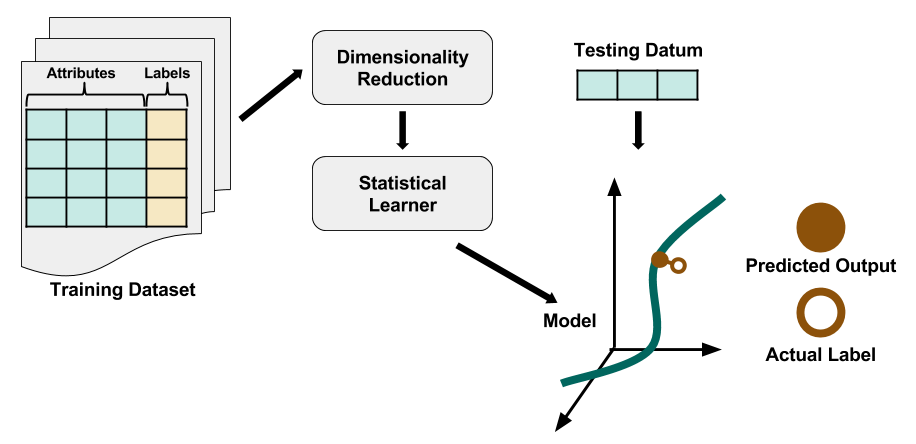
\includegraphics[width=1.15\textwidth]{./chapters/intro/SupervisedRegression.png}}
  \caption{Schematic of Regression with Machine Learning}
  \label{fig:supervised}
\end{figure}

As shown in Figure \ref{fig:supervised}, a typical (supervised) machine
learning workflow begins with a training data set, which has a number of
\textit{instances}, or rows of observations.  Each instance has some
\textit{attributes}, also referred to as \textit{features}, and a label, which
can be a categorical label or discrete/continuous values.  

The training data are then inserted into a statistical learner; this calculates
some objective, minimizes or maximizes that objective, and provides some model.
This model is typically evaluated using a testing set that has the same set of
attributes and labels (but different instances). The comparison of what the
model predicts and the actual label gives the \textit{generalization error}.
Depending on the performance and application, the model may need improvement
from more training and/or some changes in the algorithm parameters. Once the
model is performing well enough and validated, it is finalized; then a user can
provide a single instance and a value can be predicted from that. 

This study performs regression tasks using supervised learning algorithms.
Differences among the underlying mathematics of the algorithms impact the
trained models.  Therefore the algorithms used in this study will be discussed
in Section \ref{sec:algs}. Next, model selection and assessment is covered in
Section \ref{sec:selectass}.  Evaluating and optimizing algorithm performance
is discussed in Section \ref{sec:optvalid}, as well as robustly comparing
different algorithms for validation.

\subsection{Algorithms for Statistical Learning}
\label{sec:algs}
%\setlength\abovedisplayskip{2.5pt}

For relevant nuclear forensics predictions, both classification and regression
algorithms must be used.  For example, one may want to predict the reactor type
label given some measurement-based features of \gls{SNF} of an unknown source.
This would require a classification algorithm. Or perhaps the input fuel
composition is relevant to an investigation on weapons intent, so a regression
algorithm would be used. 

There are three algorithms presented in this section: \textit{k}-nearest
neighbors, decision trees, and \gls{MLL} calculations. They were chosen based
on their simplicity; this work has yet to be benchmarked using simple
algorithms so a more complex treatment of the training sets in this work would
be premature. Additionally, in part because of their simplicity, they are all
"white box" methods.  This is unique in the \gls{ML} universe, since most
algorithms create a black box model that is unable to be analyzed by a human.
The  decision trees method provides an output model that can be used to discern
behavior and understand predictions, and \textit{k}-nearest neighbors and
\gls{MLL} calculations do not create a model at all. Individual predictions can
still be analyzed, however, since the procedures are so simple. 

\subsubsection{Nearest Neighbor Methods}

Nearest neighbors classification and regression are unique algorithms in
that thay are instance-based; they do not actually generalize, but instead
track the observations in the training set.  The main metric for this algorithm
is distance (or dissimilarity) between the test sample and the closest training
sample(s) in the vicinity.  During prediction, the algorithm will calculate a
value based on the instance that is closest to the current test sample. Thus,
there is not any learning, but instead a direct comparison between an unknown
sample and the space that the training set populates. The predictions from
nearest neighbors can be quite accurate, but are highly unstable to
peturbations \cite{elements_stats}.

The process of prediction with \textit{k}-nearest neighbors is as follows.
First, the distances between the test sample and each of the training set
instances are calculated.  Most commonly the Euclidian distance is used, but
this walkthrough uses the Manhattan distance:
\begin{equation}
  d_{i} = \sum_{j=1}^{N_{feats}} |x_{j,train} - x_{j,test}|
  \label{eq:l1}
\end{equation}
where $i$ is each training set instance, and $j$ refers to each feature in the
training set.  The lowest \textit{k} $d_{i}$ are chosen. For \textit{k}-nearest
neighbors regression, the value, $y$ is predicted using the following equation.
\begin{equation}
  y(\boldsymbol{x}) = \frac{1}{k} \sum_{i=1}^{k} w_i \cdot y_i
  \label{eq:knn}
\end{equation}
where $w_{i}$ is either uniform and takes on a value of $1$ or is
distance-based and takes on a value of $1/d_{i}$ and $\boldsymbol{x}$ is the
full set of features. The regression equation averages the closest \textit{k}
neighbors for an estimate of the unknown sample.  In \textit{k}-nearest
neighbors classification, the class label $y$ is predicted using the mode of
the nearest neighbors selected using the \textit{k} smallest $d_i$, or when
$w_i$ is $1/d{i}$ the weighted mode is used to choose the predicted label.

\begin{figure}[!htb]
  \centering
  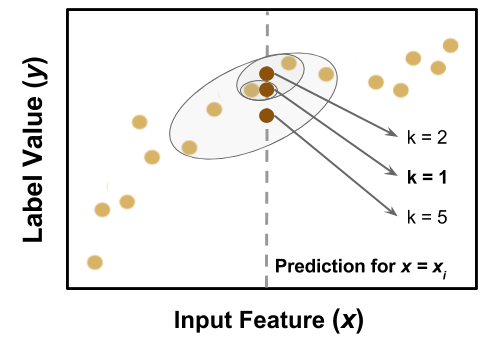
\includegraphics[width=0.8\linewidth]{./chapters/litrev/nn-fig.png}
  \caption{Schematic of \textit{k}-nearest neighbors regression, showing how 
           changing \textit{k} alters the predicted label value $y$.}
  \label{fig:nn}
\end{figure}

Figure \ref{fig:nn} provides a pictoral explanation of Equation \ref{eq:knn}
for a prediction where there is one feature. In this figure, there is a test
sample with a feature, valued at $x_i$, indicated with the grey dotted line.
The three circles represent the neighborhood given by the value of \textit{k},
and the darker dots on the line represent the reported prediction $y$ for each
choice of \textit{k}.  In this illustration, $k=1$ or $k=2$ provide a more
accurate prediction according to a visual inspection of the trend, but higher
values of $k$ can be useful, and will be discussed in Section
\ref{sec:complexity}.

\subsubsection{Decision Trees}

Decision trees are a common choice because they are simple to implement and
provide an interpretable model. However, the predictions from decision trees,
similar to \textit{k}-nearest neighbors, are unstable to peturbations.  What
follows is a highly simplified explanation of the Classification and Regression
Trees algorithm for growing decision trees, showing only the equations for
splitting criteria.  A more complete treatment can be found in Reference
\cite{elements_stats} or in the User Guide in Reference \cite{scikit}.

At their core, decision trees algorithms split the feature space into different
regions.  Decision trees are constructed by iteratively finding places in the
feature space at which to split the data to best predict a label. Some measure
of information gain (more accurately the opposite, impurity, denoted here as
$H$) is used to select a splitting criterion at each split, which maximizes
differentiation between average label values in regression or groups similar
labels together in classification.  This process continues until some
externally set stopping requirement is met, or no information gain can be made
by continuing to create splits. 

Each split creates two new nodes on the tree, where the node has to find a new
splitting criterion. In the math that follows, there are nodes given by $m$,
and a number of samples in each node given by $N_{\text{samples}, m}$. The
individual node samples are given by $i$. The impurity at the node is denoted
as $H(m)$. In classification, the node impurity can be measured by the Gini
index, where $p_{m, k}$ is the proportion of class $k$ observations at the
node:
\begin{equation}
  \begin{aligned}
    p_{m, k} &= \frac{1}{N_{\text{samples}, m}} \sum_{i=1}^{N_{\text{samples}, m}}
              I(y = k)
    \\
    H(m) &= \sum_k p_{m, k} (1 - p_{m, k})
  \end{aligned}
\end{equation}
And in regression, the node impurity $H(m)$ can be measured by the mean squared
error, where $\bar{y}_m$ is the average value of the samples in the node.
\begin{equation}
  \begin{aligned}
    \bar{y}_m &= \frac{1}{N_{\text{samples}, m}} \sum_{i=1}^{N_{\text{samples}, m}} 
                 y_{i, m}
    \\
    H(m) &= \frac{1}{N_{\text{samples}, m}} \sum_{i=1}^{N_{\text{samples}, m}}
              (y_i - \bar{y}_{i, m})^2
  \end{aligned}
\end{equation}
The splitting criterion with the lowest impurity is the one that is chosen to
make the split.  This will partition the feature space and the splitting
process will continue until a pre-defined tree size or number of samples per
node. Without a pre-defined stopping point the tree will grow until there is
one sample per node. This process can be understood more intuitively by
stuyding Figure \ref{fig:dtr}. Note that this tree was created using a maximum
tree depth of $2$ for visualization purposes in order to explain the process,
so is not indicative of a real decision tree.

\begin{figure}[!htb]
  \centering
  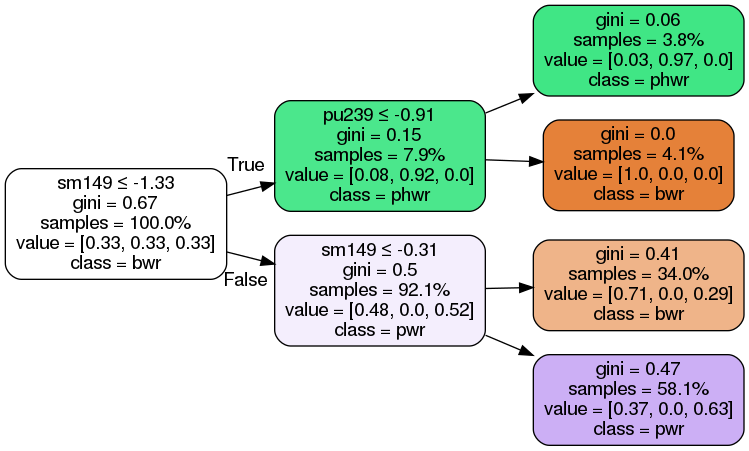
\includegraphics[width=\linewidth]{./chapters/litrev/dtree.png}
  \caption{Example of a decision tree process, where maximum tree depth was 
           limited to 2 for vizualization purposes.}
  \label{fig:dtr}
\end{figure}

In Figure \ref{fig:dtr}, the first split is determined to occur at the feature
Sm149 on whether the nuclide measurement is above a value of $-1.33$. Note that
this value is negative because of the scaling process the training set is put
through, described in Section \ref{sec:statmodel1}. The majority class at this
node is \gls{BWR} which is expected since the training set is 72\% \gls{BWR}.
The values list indicates the fraction of each class in the node, which is
alphabetically ordered \texttt{[bwr, phwr, pwr]}. It is even among the three
because the class weights were told to be balanced.  This splitting criterion
provides a Gini impurity score of 0.67, which represents the minimum Gini
impurity of all the candidate splits, but also indicates there are multiple
classes represented in this node (again, expected).  It would be 0 if there
were only one class in the node.  In the visualization, the shading of the
colors in the tree are bolder for there being a higher fraction of a single
class.

\subsubsection{Maximum Log-Likelihood Calculations}

The \gls{MLL} calulations approach applied here is based on a method developed
to do similar work \cite{mll_method, mll_validate, mll_sensitivity}.  That work
involved matching nuclear material samples based on some select measurements to
entries in a database of containing those measurements (see Section
\ref{sec:stats4nf}).  Each database entry also has a similar list of labels to
the labels being predicted in this work: reactor type, burnup, and time since
irradiation.

Interestingly, the \gls{MLL} calculations method works like \textit{k}-nearest
neighbors, where there is no model but a prediction according to the closest
match database entry.  There is one detail that differs, however. Whereas
\textit{k}-nearest neighbors minimizes distance/dissimilarity, this approach
instead maximizes similarity via a likelihood function. An "unknown" test
sample is compared against the training set using the likelihood calculation
between that sample and the training set entries.  The higher the likelihood,
the higher the probability that the database entry represents the sample. The
likelihood is in Equation \ref{eq:like}, whereas the log-likelihood is used
more often in practice, shown in Equation \ref{eq:loglike}.
\begin{equation}
  L(M|x_{test}) = \prod_i \frac{1}{\sigma_{i,train} \sqrt{2\pi}} \exp{\frac{-(x_{i,test} - x_{i,train})^2}{2 \sigma_{i,train}^2}}
  \label{eq:like}
\end{equation}
\begin{equation}
  ln(L(M|x_{test})) = \sum_i ln(\frac{1}{\sigma_{i,train} \sqrt{2\pi}}) - \frac{(x_{i,test} - x_{i,train})^2}{2 \sigma_{i,train}^2}
  \label{eq:loglike}
\end{equation}
The likelihood is a measure of the probability that a model $M$ produced the
measurements seen in the test sample, given by $L(M|x_{test})$.  In both
Equations \ref{eq:like} and \ref{eq:loglike}, $x$ refers to the set of
features, and $x_{i, test}$ and $x_{i,train}$ are the individual features for the
test sample and the training set entries, respectively. The uncertainty of the
measurement associated with each feature is represented by $\sigma_{i,train}$.



\subsection{Model Selection and Assessment}
\label{sec:selectass}
After a model is trained, the first step is model selection and assessment.
Selection is estimating model performance among a set of trained models using a
single validation set.  After one model is chosen, assessment takes place by
determining the prediction capability on new data via a previously unseen
testing set. Both selection and assessment can be done in a single step using
\textit{k}-fold cross-validation, which is described below.

\subsubsection{Sources of Error} 

In statistical learning, there are two sources of error that need to be
simultaneously minimized: bias and variance. Bias is caused by simplifications
in the model, so the error is caused by missed relationships in the data; an
underfit model is due to high bias.  Variance is caused by including random
noise in the model, so the error is caused by oversensitivity to that noise; an
overfit model is due to high variance. 

%%%%%%%%%%%%%%%%%%%%%%%%%%%%%%%%%%%%%%%%%%%%%%%%%%%%%%%%%%%%
%%%%%%%%%%%%%%%%%%%%%%%%%%%%%%%%%%%%%%%%%%%%%%%%%%%%%%%%%%%%
Include math or just reference it?
Talk about irreducible error too?
%%%%%%%%%%%%%%%%%%%%%%%%%%%%%%%%%%%%%%%%%%%%%%%%%%%%%%%%%%%%
%%%%%%%%%%%%%%%%%%%%%%%%%%%%%%%%%%%%%%%%%%%%%%%%%%%%%%%%%%%%

\begin{figure}[!htb]
  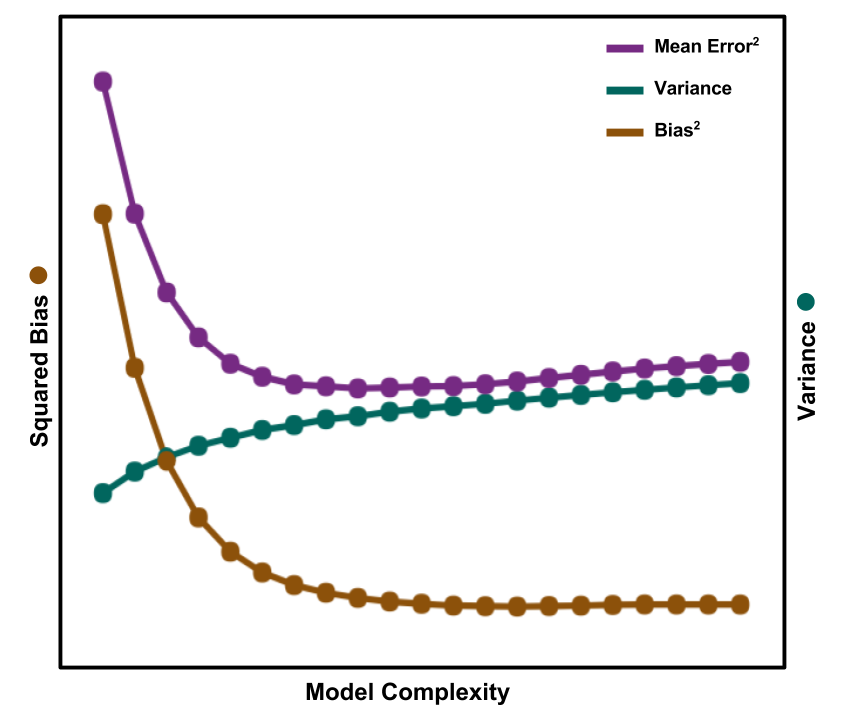
\includegraphics[width=\linewidth]{./chapters/litrev/BVtradeoff.png}
  \caption{Total prediction error comprised of bias and variance}
  \label{fig:bvtradeoff}
\end{figure}

As shown in Figure \ref{fig:bvtradeoff}, there is a minimum in the total error,
showing that there is a tradeoff between the bias and variance. Some bias is
desired in order to generalize to future unknown data. But some variance is
also positive for the model because it captures the relationships in the data
that the bias counteracts. 

\subsubsection{Types of Error}

While the sources of the model prediction error are well known, the creation of
a statistically learned model is a hidden process. Although the model emerges
from a black box, there are ways to evaluate the generalization (i.e.,
prediction) capability of it.  This is done by removing a small portion of the
data for use as a testing set.  The rest of the data set is known as the
training set and is used to train a model. After training, the test set is used
to test the model.  

The generalization error is typically referred to as the \textit{testing
error}, as it is measuring the ability of the model to predict future cases
that were not introduced in the training phase (i.e., the testing set entries).
Next, the \textit{training error} is provided by comparing the model
predictions to the training set, as the model would likely be smoother than the
potential noise the training set would include. This is useful to determine the
fitness of the model, the application of which is discussed below in Section
\ref{sec:optvalid}.

Although one could just train and test their model, there is a way to test the
model while still in the training phase. A testing set that would be used
during training to give feedback, a \textit{cross-validation} set, can provide
a faster convergence to a satisfactory model. As shown in Figure
\ref{fig:cverror}, this can be done by splitting the data set into three
groups: a large training set, a small cross-validation set, and a small testing
set. 

\begin{figure}[!htb]
  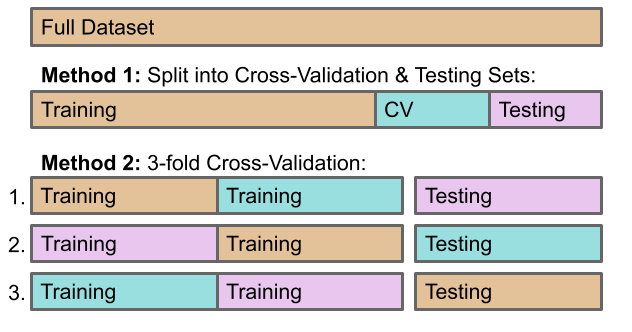
\includegraphics[width=\linewidth]{./chapters/litrev/cverror.png}
  \caption{Illustration of how a dataset can be split up for model evaluation}
  \label{fig:cverror}
\end{figure}

However, in practice, multiple rounds of cross-validation steps are used,
referred to as \textit{k-fold cross-validation}. This allows a user to use all
data entries as a testing entry once.  As illustrated in \ref{fig:cverror},
this splits the dataset into \textit{k} subsets. One set is designated as the
testing set, and a model is trained with the rest. Following the first training
phase, another begins, this time with a different subset as the testing set.
This process is performed \textit{k} times to give \textit{k} models, and the
models are then averaged, providing an additional level of model validation
than can be achieved with a single testing set.



\subsection{Model Optimization and Validation}
\label{sec:optvalid}
It is unlikely to have a model perform as one expects the first time. There are
therefore a few techniques for optimizing the performance. It should be noted
that much of the discussion here and in Section \ref{sec:valid} focuses on
the diagnostics aspect rather than the validation aspect of these techniques.
In practice, these are used for both purposes, but in this work the formal
comparison of model performance will be used, introduced and detailed in
Sections \ref{sec:invcompare} and \ref{sec:modelcompare}, respectively. 

However, the increase in performance from over-optimization could be linked to
the training set performance and might not generalize outside of the specific
type of input data used.  A workaround for this scenario is to obtain more data
for the set or to obtain a completely different data set altogether. 

\subsubsection{Training Set Size}

The first diagnostic plot for optimizing the model performance is called a
\textit{learning curve}, which provides information about the bias-variance
tradeoff with respect to the data set size. More specifically, learning curves
compare the training and cross-validation errors to the size of the training
set (i.e., number of instances in the training set). This is done by randomly
selecting a percentage of the the training set, inputting that into a
statistical learner, and tabulating the error of the learned model. 

Typically, a learning curve will look somewhat like one of the three examples
in Figure \ref{fig:learning}\footnote{These schematics are based on hand-drawn
diagrams by Ritchie Ng on http://www.ritchieng.com/applying-machine-learning/}.
A learning curve tests the model for high bias or high variance, which can
correspond to an undefit or overfit model, respectively. 

\begin{figure}[!hp]
  \centering
  \begin{subfigure}[h]{0.65\linewidth}
    \centering
    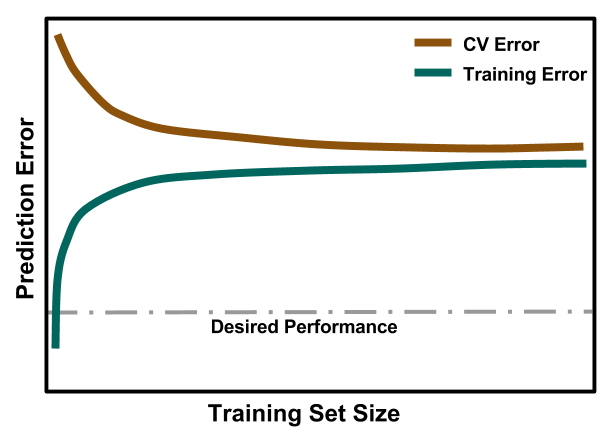
\includegraphics[width=\linewidth]{./chapters/litrev/LearningCurve-bias.png}
    \caption{High bias}
    \label{fig:bias}
  \end{subfigure}
  \begin{subfigure}[h]{0.65\linewidth}
    \centering
    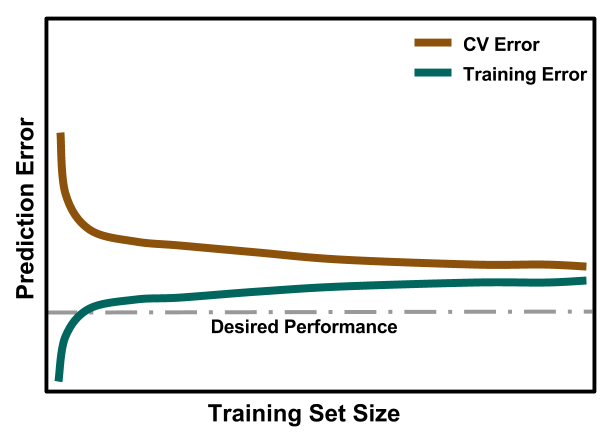
\includegraphics[width=\linewidth]{./chapters/litrev/LearningCurve-ideal.png}
    \caption{Ideal}
    \label{fig:ideal}
  \end{subfigure}
  \begin{subfigure}[h]{0.65\linewidth}
    \centering
    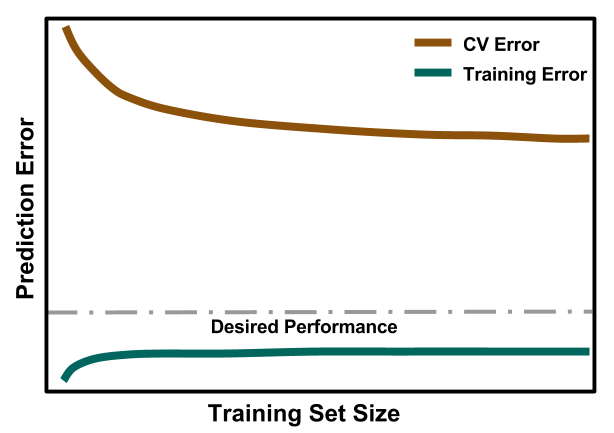
\includegraphics[width=\linewidth]{./chapters/litrev/LearningCurve-variance.png}
    \caption{High variance}
    \label{fig:variance}
  \end{subfigure}
  \caption{Learning curves for three training scenarios}
  \label{fig:learning}
\end{figure}

Figure \ref{fig:bias} suggests underfitting because the model is missing
important features in the data. It is characterized by a small gap between the
curves but high overall errors. The cross-validation error remains consistently
high and the training error increases drastically with increasing data, since
it is not generalizing well. 

Figure \ref{fig:variance} suggests overfitting because the model has too much
sensitivity to variations in the data. It is characterized by a very large gap
between the curves. It has an extremely low training error, as it has taken
into account every detail of the training set, but a high cross-validation
error because it cannot generalize beyond the testing set. 

Figure \ref{fig:ideal} is an example of a more ideal model fit. It is
characterized by a small gap between the two errors, and they are at a
reasonable level with respect to the desired performance.  The training error
should increase with respect to the training set size due to a larger amount of
bias (preventing overfitting). But the cross-validation error should decrease
quickly with respect to the training set size due to being close to the minimum
of the bias-variance tradeoff. 

\subsubsection{Model Complexity}

After ensuring the appropriate training set size is selected, the models must
be further optimized using \textit{validation curves}.  These provide
information on the bias-variance tradeoff with respect to model complexity. Two
main factors affecting model complexity can cause the model to be under- or
overfit to the data: number of features in the data set and algorithm
parameters that vary the regularization.

\begin{figure}[!htb]
  \centering
  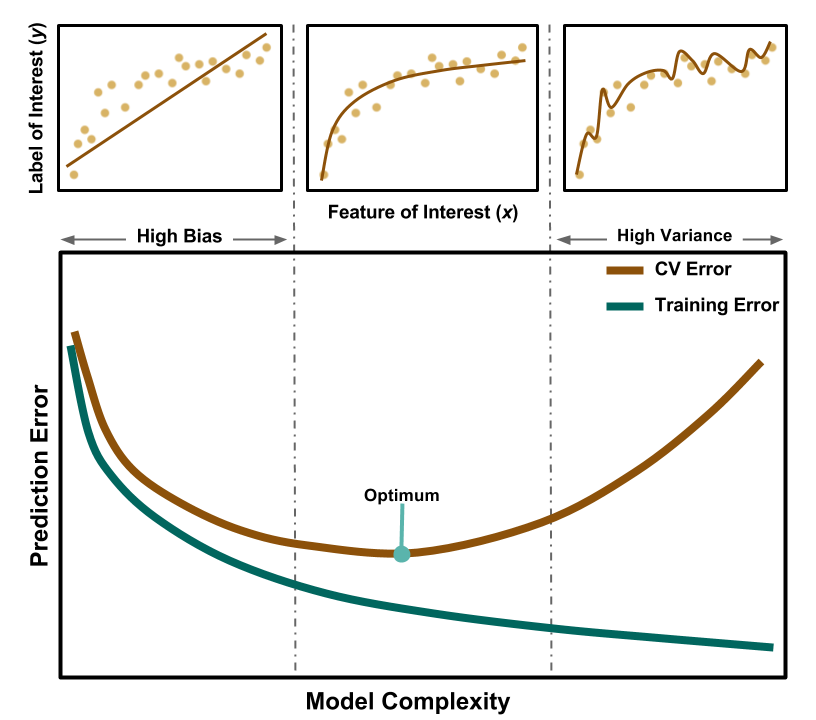
\includegraphics[width=1.05\linewidth]{./chapters/litrev/ValidationCurve.png}
  \caption{Validation curve showing examples of different fittings}
  \label{fig:validation}
\end{figure}

Figure \ref{fig:validation} adapted from Ref. \cite{elements_stats} shows the
optimum as the minimum of the cross-validation error curve. There is some gap
between it and the training error, much larger than the left side of the plot
and much smaller than the right.  The plot above is a visualization of a
decently fit model.  The left region is marked by both errors being quite high,
and above is an  illustration of how an underfit plot (high bias) could provide
high errors. The right region shows the training error being quite low but the
cross-validation error being high. The diagram above shows that it is obvious
how the training error would be negligible, but generalizing beyond that
probably will not yield accurate results. 

In practice, plotting learning and validation curves can be iterative. But as
previously mentioned, too many optimizations will result in a poorly performing
model when exposed to data outside of the training set.

\subsubsection{Comparison of Methods}
\label{sec:invcompare}

In addition to evaluating a single learned model, it will be beneficial to
compare models. This can be done using Bayesian inference as discussed in
Section \ref{sec:inverse}.  Equations \ref{eq:bayes} and \ref{eq:bayes_words}
show that there are three values to obtain to calculate a posterior
probability, i.e., the probability of a parameter estimated from a
machine-learned model being correct: the likelihood, the prior probability, and
the marginal likelihood. 

The posterior probability represents the solution to an \textit{inverse}
problem, where model parameters are predicted from some given measurement
values. It is not directly computable and thus the remaining probabilities
discussed below indirectly allow its computation.  In this context, it is the
probability that a predicted reactor parameter from a chosen method is correct
given input based on an \gls{SNF} recipe.  For example, it is the probability
that a plutonium-239 concentration of $y\%$ is attributed to a uranium oxide
fuel in a \gls{BWR} with a burnup of $x\ GWd/MTU$.  Most inverse problems are
\textit{ill-posed}, usually because the solution is not guaranteed to be
unique. The posterior probabilities compared across methods will provide the
most probable correct answer. This will reveal the superior method versus
others that have lower posterior probabilities. \cite{inverse_theory}

The likelihood represents the solution to a \textit{forward} problem, where
measurement values are predicted from some given model parameters.  In this
context, this is calculated from the instances in the training data set.  The
likelihood is the probability that the output \gls{SNF} composition of a
simulation is correct given the input of reactor operation parameters.  In
practice, it will be calculated from a large number of forward simulations
using \gls{ORIGEN}, i.e., the training data set. For example, this would be the
probability that uranium oxide fuel from a \gls{BWR} having a burnup of $x\
GWd/MTU$ contains $y\%$ of plutonium-239.

The prior probability represents the spread of plausible model parameters, so
it is a hypothesis based on the breadth of the model space with no evidence
provided.  In other words, it is given by model parametertization from a number
of potential sources.  One method is expert-elicited values. Another is a
predicted model from some established theory or previously known relationship,
e.g., empirical relations between isotopic ratios and certain reactor
parameters or a direct calculation of the reactor parameters. In this context,
it is obtained from the estimated model parameters from a given statistical
model.  For example, it is the probability that a model from \gls{SVR} predicts
a burnup of $x\ GWd/MTU$ for uranium oxide fuel from a \gls{BWR} with no other 
direct measurements provided.

The marginal likelihood represents the spread of plausible measurements, so it
is based on the breath of the data space with no model-based information
provided.  In practice, however, it is calculated by summing the joint
probabilities of all possible model parameter hypotheses and measurements. This
in essence provides a normalization constant.  Thus, the marginal likelihood is
only needed for absolute posterior probability calculations; it does not affect
the relative probabilities, which are all that is needed for model comparison
\cite{inverse_theory}. 

For reference, Table \ref{tbl:bayes} is a summary of the Bayes' theorem
components described above as related to this work.

\begin{table}[!hp]
  \centering
  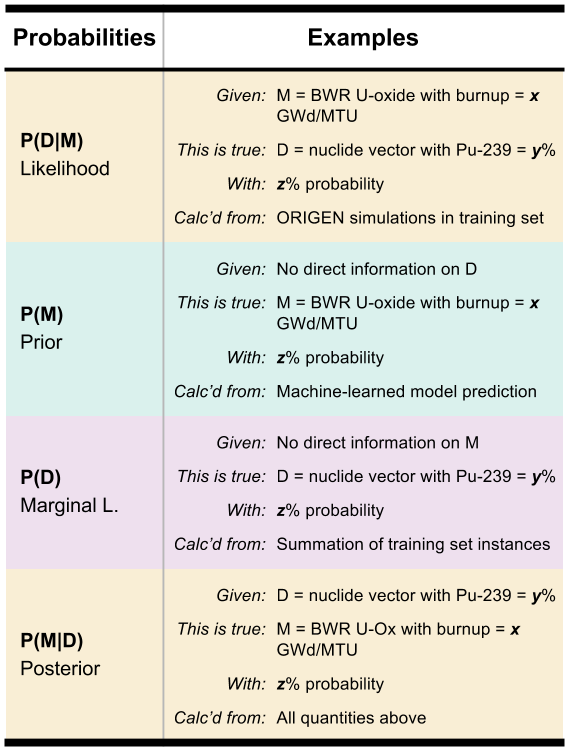
\includegraphics[width=\linewidth]{./chapters/litrev/bayes.png}
  \caption{Summary of contextual explanations of Bayes theorem components}
  \label{tbl:bayes}
\end{table}




\section{Computational Methods}
\label{sec:fcsim}
There can be a large number of computational tools within a given field of
study.  They are typically developed with one aspect of analysis in mind, so
one must understand the simplifying assumptions the developers made for their
purposes. Thus, choosing a computational tool is not always obvious. Thus, this
section both introduces and defends the choices for the various experimental
components.

\subsection{Fuel Cycle Simulation}

Nuclear fuel cycle studies involve tracking the material flow of nuclear fuel.
This can be anywhere from mining to waste management, or focus on a process
step anywhere in between. Fuel cycle studies are not necessarily
nuclear-specific. They can be used to evaluate, e.g., economic predictions,
environmental impact, transportation planning, etc.  In order to draw
conclusions from these studies, it is common to use a nuclear fuel cycle
simulator that tracks the quantities of interest. These allow the comparison of
different fuel types, reactor technologies, material processing steps, etc. 

As mentioned, there are simplifications researchers need to make in order to
experiment in a controlled way. Fuel cycle simulators are built for specific
needs as well and also must remove complicating factors that are generally less
relevant to the study.  For example, one tool might be suited well to
large-scale systems analysis with little nuclear physics included in the
models, and another might focus on detailed isotopics within a system to track
plutonium isotopes.

\todo{more needed?}

Because a large portion of a nuclear forensics investigation relies on
measuring isotopics, \gls{ORIGEN-ARP} \cite{origen} within the SCALE code
system was chosen for its physically detailed models. \gls{ORIGEN} calculates
time-dependent nuclide concentrations (or quantities derived from these) that
result from activation and depletion calculations. The physics (i.e., neutron
transport and decay) calculations are carried out in other SCALE modules that
solve the depletion equations.  This generates libraries for \gls{ORIGEN} that
include the probabilities of reaction (i.e., cross sections) for the system.

To obtain an \gls{SNF} recipe from a reactor simulation, \gls{ORIGEN} uses the
desired input power generation with the cross section library to calculate a
flux, the resulting depletion, and the end composition (i.e., isotopics,
nuclide vector).  Another output is decay; the composition is computed using
decay equations with nuclear data \cite{endf}. These compositions provide
source terms for other calculations, such as decay emission spectra from
neutrons, or alpha, beta, gamma rays, which use the same resource for nuclear
data. Other quantities like activity, decay heat, or radiological hazard
factors are also an option.

\gls{ORIGEN-ARP} allows users to access a wider range of simulations by
interpolating between the already calculated libraries for a wide array of
reactors instead of creating new libraries.  It is known to be validated for
\gls{LWR} \gls{SNF} \cite{lwr_valid}. Additionally, recycled \gls{SNF} in the
form of mixed oxide fuel has been benchmarked with the relevant reactors
\cite{mox_valid}.  Thus, given an initial material composition, some reactor
operation parameters, and a reactor type, one can quickly perform many
different nuclear reactor simulations and obtain \gls{SNF} recipes.

\subsection{Statistics Toolkit}

The statistics toolkit chosen for this work is scikit-learn \cite{scikit}, a
machine learning package in python.  Virtually all modern machine learning
toolkits will have acceptably fast and reliable algorithms, but the use of
python provides a platform for seamless integration of all the tools in the
workflow. 

\subsection{Computational Gamma Spectra}

Although the data modification shown later in Section \ref{sec:inforeduc} does
not use any standalone tool, the code \gls{GADRAS} \cite{gadras} developed at
Sandia National Laboratories will provide information reduction in a physically
valid manner.  Test studies will be carried out using the gamma spectra
available from \gls{ORIGEN} simulations, but the detector response will need to
be varied more than this tool can provide. Thus, given the nuclide vectors from
\gls{ORIGEN}, \gls{GADRAS} computationally generates gamma spectra from the
gamma energies and a chosen \gls{DRF}. This will enable a more robust study of 
statistical performance with respect to information reduction.



\section{Applications of Statistical Methods to Nuclear Forensics Analysis}
\label{sec:stats4nf}
I'm the lit review section on previous applied ML work in the NF field.

\subsection{Special Nuclear Materials Studied}

The review on nf for the whole fuel cycle is useful here, perhaps. This is also 
important when I discuss my risk management section later. 

\subsection{Statistical Methods Employed}

Very short details from lit review outline and success rates should be 
discussed here



\chapter{Demonstration}
\label{ch:demo}

Fill me in, yo.

\section{Introduction}
\label{sec:demointro}

Need to figure out what to put here and what goes in intro. Also workflow
details repeated if it's in the intro?

\section{Experimental Components}
%Training data and more ORIGEN stuff 
This work begins by simulating the training and test sets described in ref
(cite Dayman). As with the previous work, this will be done using SCALE 6.2
\todo{cite}. Specifically, the ARP module of the activation and depletion code
ORIGEN was used. \todo{add deets and citations}

\todo{show table of training set space}
The parameters of the training set are defined as follows. A smaller burnup
than is typical for spent fuel from a commercial reactor is used in the
previous work likely because stolen fuel pins for weapons use would not likely
be at the end of their lifetime, as the plutonium of interest has decreased by
then. A truly i.i.d. training set would go beyond this, but this is purely for
demonstration with a single use case in mind. 

\todo{show table of test set space}
The previous work also used an external test set, designed to have values in
between the trained values of burnup. This is implemented in this study but it
is expected that cross-validation will better indicate the model performance.
More specifically, using k-fold cross-validation is a common method to use in
the application of machine learning to create more confidence in the resulting
model. \todo{either explain or cite cross validation next}

%DRF and Iso ID
detector response function and iso ID

%Demonstrate success with iso only
here's some awesome success with only isotopes


\section{Comparison to Other Work}
\label{sec:compare}

\subsection{Information Reduction}

This study evaluates the impact of randomly introduced error of varying amounts
on the ability of the algorithms to correctly predict the burnup. Thus, first
investigated are the three algorithms with no error introduced, and next with
the random errors applied uniformly to each nuclide vector. Since error in a
nuclide vector is not random, in fact it is systematic and dependent on a
number of known sources of uncertainty, the next study will introduce error by
limiting the nuclides to only those that can be measured with a gamma
spectrometer (future work).

\section{Expanding the Training Set}
\label{sec:newtrain}

BeepBop


\begin{frame}
  \frametitle{Computational Methods}
  \begin{figure}[h!]
    \centering
    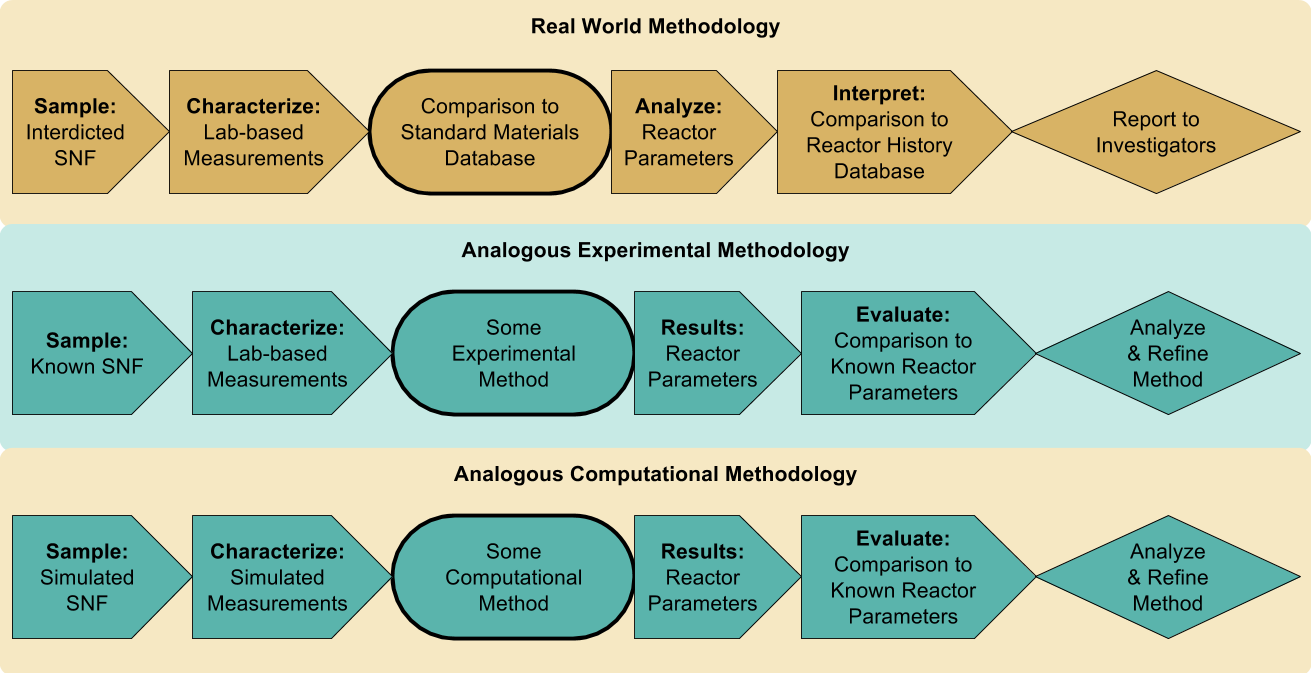
\includegraphics[width=0.9\textwidth]{./figures/ForensicsWorkflows.png}
    \caption{Nuclear forensics research: physical, experimental, and computational}
  \end{figure}
\end{frame}

\begin{frame}
  \frametitle{Computational Methods}
  \begin{figure}[h!]
    \centering
    \includegraphics[width=0.9\textwidth]{./figures/CompStatForensicsWorkflow.png}
    \caption{Comparison of two different computational approaches}
  \end{figure}
\end{frame}

\begin{frame}
  \frametitle{Statistical Methods}
  \begin{minipage}{0.5\textwidth}
    \begin{figure}
      \centering
      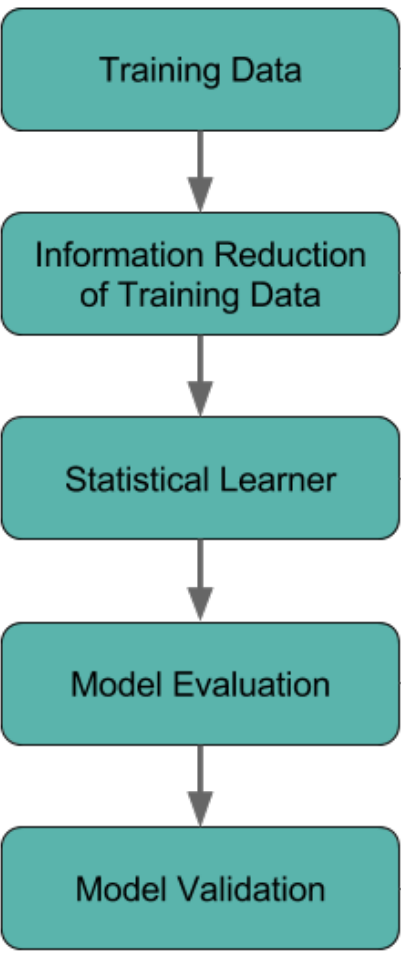
\includegraphics[height=0.6\textheight]{./figures/statmethodology.png}
      \caption{Workflow of a  methodology using statistical models}
    \end{figure}
  \end{minipage}%
  \begin{minipage}{0.5\textwidth}
    \begin{itemize}
      \item Training data: large set of SNF measurements
      \begin{itemize}
        \item Labels (e.g., burnup)
        \item Features (e.g., nuclide concs)
        \item Instances (individual SNF recipe)
      \end{itemize}
      \item Statistical learner
      \begin{itemize}
        \item Machine learning algorithms
        \item Algorithm parameters
        \item Predict label of new instance
      \end{itemize}
      \item Model evaluation
      \begin{itemize}
        \item Diagnostic curves
        \begin{itemize}
          \item Learning curves
          \item Validation curves
        \end{itemize}
        \item Prediction error
        \begin{itemize}
          \item Bias versus variance
          \item Generalizability
        \end{itemize}
      \end{itemize}
    \end{itemize}
  \end{minipage}
\end{frame}

\begin{frame}
  \frametitle{Statistical Methods}
  \begin{figure}[h!]
    \centering
    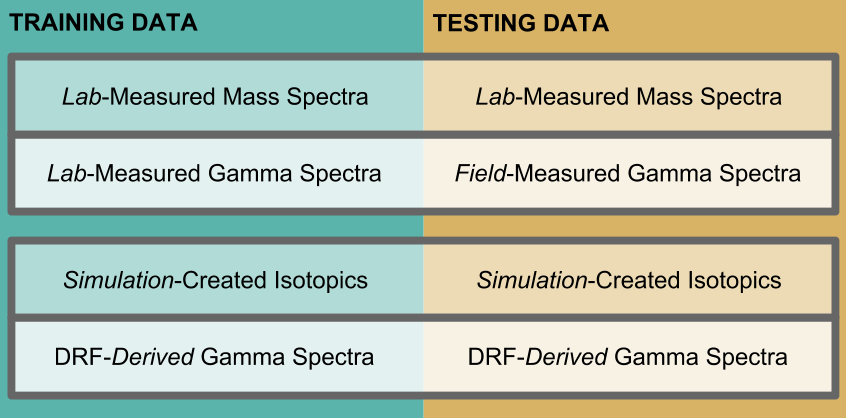
\includegraphics[width=0.75\textwidth]{./figures/proposal.png}
    \caption{Illustration of data set modularity}
  \end{figure}
\end{frame}



%% Do you have appendices?  If so, add them here, just like chapters.
% \begin{appendices}
% \include{backmatter/appendix1}
% \end{appendices}

%% McBride is a very nice style (some version is included in this distribution)
\bibliographystyle{mcbride}
\bibliography{dissertation}

\end{document}
